\documentclass[twoside]{book}

% Packages required by doxygen
\usepackage{fixltx2e}
\usepackage{calc}
\usepackage{doxygen}
\usepackage[export]{adjustbox} % also loads graphicx
\usepackage{graphicx}
\usepackage[utf8]{inputenc}
\usepackage{makeidx}
\usepackage{multicol}
\usepackage{multirow}
\PassOptionsToPackage{warn}{textcomp}
\usepackage{textcomp}
\usepackage[nointegrals]{wasysym}
\usepackage[table]{xcolor}

% Font selection
\usepackage[T1]{fontenc}
\usepackage[scaled=.90]{helvet}
\usepackage{courier}
\usepackage{amssymb}
\usepackage{sectsty}
\renewcommand{\familydefault}{\sfdefault}
\allsectionsfont{%
  \fontseries{bc}\selectfont%
  \color{darkgray}%
}
\renewcommand{\DoxyLabelFont}{%
  \fontseries{bc}\selectfont%
  \color{darkgray}%
}
\newcommand{\+}{\discretionary{\mbox{\scriptsize$\hookleftarrow$}}{}{}}

% Page & text layout
\usepackage{geometry}
\geometry{%
  a4paper,%
  top=2.5cm,%
  bottom=2.5cm,%
  left=2.5cm,%
  right=2.5cm%
}
\tolerance=750
\hfuzz=15pt
\hbadness=750
\setlength{\emergencystretch}{15pt}
\setlength{\parindent}{0cm}
\setlength{\parskip}{3ex plus 2ex minus 2ex}
\makeatletter
\renewcommand{\paragraph}{%
  \@startsection{paragraph}{4}{0ex}{-1.0ex}{1.0ex}{%
    \normalfont\normalsize\bfseries\SS@parafont%
  }%
}
\renewcommand{\subparagraph}{%
  \@startsection{subparagraph}{5}{0ex}{-1.0ex}{1.0ex}{%
    \normalfont\normalsize\bfseries\SS@subparafont%
  }%
}
\makeatother

% Headers & footers
\usepackage{fancyhdr}
\pagestyle{fancyplain}
\fancyhead[LE]{\fancyplain{}{\bfseries\thepage}}
\fancyhead[CE]{\fancyplain{}{}}
\fancyhead[RE]{\fancyplain{}{\bfseries\leftmark}}
\fancyhead[LO]{\fancyplain{}{\bfseries\rightmark}}
\fancyhead[CO]{\fancyplain{}{}}
\fancyhead[RO]{\fancyplain{}{\bfseries\thepage}}
\fancyfoot[LE]{\fancyplain{}{}}
\fancyfoot[CE]{\fancyplain{}{}}
\fancyfoot[RE]{\fancyplain{}{\bfseries\scriptsize Generated by Doxygen }}
\fancyfoot[LO]{\fancyplain{}{\bfseries\scriptsize Generated by Doxygen }}
\fancyfoot[CO]{\fancyplain{}{}}
\fancyfoot[RO]{\fancyplain{}{}}
\renewcommand{\footrulewidth}{0.4pt}
\renewcommand{\chaptermark}[1]{%
  \markboth{#1}{}%
}
\renewcommand{\sectionmark}[1]{%
  \markright{\thesection\ #1}%
}

% Indices & bibliography
\usepackage{natbib}
\usepackage[titles]{tocloft}
\setcounter{tocdepth}{3}
\setcounter{secnumdepth}{5}
\makeindex

% Hyperlinks (required, but should be loaded last)
\usepackage{ifpdf}
\ifpdf
  \usepackage[pdftex,pagebackref=true]{hyperref}
\else
  \usepackage[ps2pdf,pagebackref=true]{hyperref}
\fi
\hypersetup{%
  colorlinks=true,%
  linkcolor=blue,%
  citecolor=blue,%
  unicode%
}

% Custom commands
\newcommand{\clearemptydoublepage}{%
  \newpage{\pagestyle{empty}\cleardoublepage}%
}

\usepackage{caption}
\captionsetup{labelsep=space,justification=centering,font={bf},singlelinecheck=off,skip=4pt,position=top}

%===== C O N T E N T S =====

\begin{document}

% Titlepage & ToC
\hypersetup{pageanchor=false,
             bookmarksnumbered=true,
             pdfencoding=unicode
            }
\pagenumbering{alph}
\begin{titlepage}
\vspace*{7cm}
\begin{center}%
{\Large Chess \\[1ex]\large 1.\+1 }\\
\vspace*{1cm}
{\large Generated by Doxygen 1.8.12}\\
\end{center}
\end{titlepage}
\clearemptydoublepage
\pagenumbering{roman}
\tableofcontents
\clearemptydoublepage
\pagenumbering{arabic}
\hypersetup{pageanchor=true}

%--- Begin generated contents ---
\chapter{Namespace Index}
\section{Packages}
Here are the packages with brief descriptions (if available)\+:\begin{DoxyCompactList}
\item\contentsline{section}{\hyperlink{namespacechess_game}{chess\+Game} }{\pageref{namespacechess_game}}{}
\end{DoxyCompactList}

\chapter{Hierarchical Index}
\section{Class Hierarchy}
This inheritance list is sorted roughly, but not completely, alphabetically\+:\begin{DoxyCompactList}
\item \contentsline{section}{chess\+Game.\+Chess\+Board}{\pageref{classchess_game_1_1_chess_board}}{}
\item \contentsline{section}{chess\+Game.\+Game\+Play}{\pageref{classchess_game_1_1_game_play}}{}
\item \contentsline{section}{chess\+Game.\+Piece}{\pageref{classchess_game_1_1_piece}}{}
\begin{DoxyCompactList}
\item \contentsline{section}{chess\+Game.\+Bishop}{\pageref{classchess_game_1_1_bishop}}{}
\item \contentsline{section}{chess\+Game.\+King}{\pageref{classchess_game_1_1_king}}{}
\item \contentsline{section}{chess\+Game.\+Knight}{\pageref{classchess_game_1_1_knight}}{}
\item \contentsline{section}{chess\+Game.\+Pawn}{\pageref{classchess_game_1_1_pawn}}{}
\item \contentsline{section}{chess\+Game.\+Queen}{\pageref{classchess_game_1_1_queen}}{}
\item \contentsline{section}{chess\+Game.\+Rook}{\pageref{classchess_game_1_1_rook}}{}
\end{DoxyCompactList}
\item \contentsline{section}{chess\+Game.\+Tests\+One}{\pageref{classchess_game_1_1_tests_one}}{}
\end{DoxyCompactList}

\chapter{Class Index}
\section{Class List}
Here are the classes, structs, unions and interfaces with brief descriptions\+:\begin{DoxyCompactList}
\item\contentsline{section}{\hyperlink{classchess_game_1_1_bishop}{chess\+Game.\+Bishop} }{\pageref{classchess_game_1_1_bishop}}{}
\item\contentsline{section}{\hyperlink{classchess_game_1_1_chess_board}{chess\+Game.\+Chess\+Board} }{\pageref{classchess_game_1_1_chess_board}}{}
\item\contentsline{section}{\hyperlink{classchess_game_1_1_game_play}{chess\+Game.\+Game\+Play} }{\pageref{classchess_game_1_1_game_play}}{}
\item\contentsline{section}{\hyperlink{classchess_game_1_1_king}{chess\+Game.\+King} }{\pageref{classchess_game_1_1_king}}{}
\item\contentsline{section}{\hyperlink{classchess_game_1_1_knight}{chess\+Game.\+Knight} }{\pageref{classchess_game_1_1_knight}}{}
\item\contentsline{section}{\hyperlink{classchess_game_1_1_pawn}{chess\+Game.\+Pawn} }{\pageref{classchess_game_1_1_pawn}}{}
\item\contentsline{section}{\hyperlink{classchess_game_1_1_piece}{chess\+Game.\+Piece} }{\pageref{classchess_game_1_1_piece}}{}
\item\contentsline{section}{\hyperlink{classchess_game_1_1_queen}{chess\+Game.\+Queen} }{\pageref{classchess_game_1_1_queen}}{}
\item\contentsline{section}{\hyperlink{classchess_game_1_1_rook}{chess\+Game.\+Rook} }{\pageref{classchess_game_1_1_rook}}{}
\item\contentsline{section}{\hyperlink{classchess_game_1_1_tests_one}{chess\+Game.\+Tests\+One} }{\pageref{classchess_game_1_1_tests_one}}{}
\end{DoxyCompactList}

\chapter{File Index}
\section{File List}
Here is a list of all files with brief descriptions\+:\begin{DoxyCompactList}
\item\contentsline{section}{chess\+Game/\hyperlink{_bishop_8java}{Bishop.\+java} }{\pageref{_bishop_8java}}{}
\item\contentsline{section}{chess\+Game/\hyperlink{_chess_board_8java}{Chess\+Board.\+java} }{\pageref{_chess_board_8java}}{}
\item\contentsline{section}{chess\+Game/\hyperlink{_game_play_8java}{Game\+Play.\+java} }{\pageref{_game_play_8java}}{}
\item\contentsline{section}{chess\+Game/\hyperlink{_king_8java}{King.\+java} }{\pageref{_king_8java}}{}
\item\contentsline{section}{chess\+Game/\hyperlink{_knight_8java}{Knight.\+java} }{\pageref{_knight_8java}}{}
\item\contentsline{section}{chess\+Game/\hyperlink{_pawn_8java}{Pawn.\+java} }{\pageref{_pawn_8java}}{}
\item\contentsline{section}{chess\+Game/\hyperlink{_piece_8java}{Piece.\+java} }{\pageref{_piece_8java}}{}
\item\contentsline{section}{chess\+Game/\hyperlink{_queen_8java}{Queen.\+java} }{\pageref{_queen_8java}}{}
\item\contentsline{section}{chess\+Game/\hyperlink{_rook_8java}{Rook.\+java} }{\pageref{_rook_8java}}{}
\item\contentsline{section}{chess\+Game/\hyperlink{_tests_one_8java}{Tests\+One.\+java} }{\pageref{_tests_one_8java}}{}
\end{DoxyCompactList}

\chapter{Namespace Documentation}
\hypertarget{namespacechess_game}{}\section{Package chess\+Game}
\label{namespacechess_game}\index{chess\+Game@{chess\+Game}}
\subsection*{Classes}
\begin{DoxyCompactItemize}
\item 
class \hyperlink{classchess_game_1_1_bishop}{Bishop}
\item 
class \hyperlink{classchess_game_1_1_chess_board}{Chess\+Board}
\item 
class \hyperlink{classchess_game_1_1_game_play}{Game\+Play}
\item 
class \hyperlink{classchess_game_1_1_king}{King}
\item 
class \hyperlink{classchess_game_1_1_knight}{Knight}
\item 
class \hyperlink{classchess_game_1_1_pawn}{Pawn}
\item 
class \hyperlink{classchess_game_1_1_piece}{Piece}
\item 
class \hyperlink{classchess_game_1_1_queen}{Queen}
\item 
class \hyperlink{classchess_game_1_1_rook}{Rook}
\item 
class \hyperlink{classchess_game_1_1_tests_one}{Tests\+One}
\end{DoxyCompactItemize}

\chapter{Class Documentation}
\hypertarget{classchess_game_1_1_bishop}{}\section{chess\+Game.\+Bishop Class Reference}
\label{classchess_game_1_1_bishop}\index{chess\+Game.\+Bishop@{chess\+Game.\+Bishop}}
Inheritance diagram for chess\+Game.\+Bishop\+:\begin{figure}[H]
\begin{center}
\leavevmode
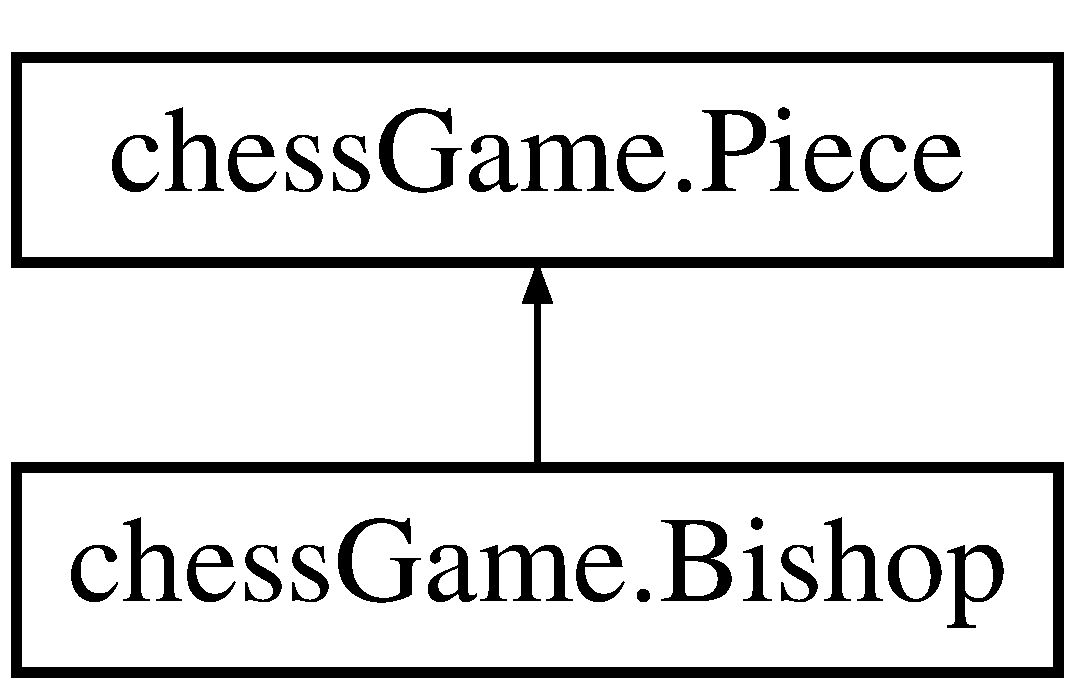
\includegraphics[height=2.000000cm]{classchess_game_1_1_bishop}
\end{center}
\end{figure}
\subsection*{Public Member Functions}
\begin{DoxyCompactItemize}
\item 
\hyperlink{classchess_game_1_1_bishop_a0e087cf48b5025c9af2fae0e6ef0c36c}{Bishop} (int \hyperlink{classchess_game_1_1_piece_aeb2d3374492005d799aa6b7b85be40e7}{x}, int \hyperlink{classchess_game_1_1_piece_a56e4d8d18eca3fd03a6bd5d6112d6359}{y}, \hyperlink{classchess_game_1_1_piece_ad5117cbbbaebf3a27c4f3c2bcbd6678b}{color} \hyperlink{classchess_game_1_1_piece_ad5117cbbbaebf3a27c4f3c2bcbd6678b}{color}, \hyperlink{classchess_game_1_1_piece_a1370c7f61581a1b72fa8ac2fd1af70a2}{type} \hyperlink{classchess_game_1_1_piece_a1370c7f61581a1b72fa8ac2fd1af70a2}{type})
\item 
boolean \hyperlink{classchess_game_1_1_bishop_a93e6dd0e281ab29a95768a09424a297c}{check\+Destination} (int \hyperlink{classchess_game_1_1_piece_aeb2d3374492005d799aa6b7b85be40e7}{x}, int \hyperlink{classchess_game_1_1_piece_a56e4d8d18eca3fd03a6bd5d6112d6359}{y}, int turn, \hyperlink{classchess_game_1_1_chess_board}{Chess\+Board} board)
\end{DoxyCompactItemize}


\subsection{Constructor \& Destructor Documentation}
\hypertarget{classchess_game_1_1_bishop_a0e087cf48b5025c9af2fae0e6ef0c36c}{}\label{classchess_game_1_1_bishop_a0e087cf48b5025c9af2fae0e6ef0c36c} 
\index{chess\+Game\+::\+Bishop@{chess\+Game\+::\+Bishop}!Bishop@{Bishop}}
\index{Bishop@{Bishop}!chess\+Game\+::\+Bishop@{chess\+Game\+::\+Bishop}}
\subsubsection{\texorpdfstring{Bishop()}{Bishop()}}
{\footnotesize\ttfamily chess\+Game.\+Bishop.\+Bishop (\begin{DoxyParamCaption}\item[{int}]{x,  }\item[{int}]{y,  }\item[{\hyperlink{classchess_game_1_1_piece_ad5117cbbbaebf3a27c4f3c2bcbd6678b}{color}}]{color,  }\item[{\hyperlink{classchess_game_1_1_piece_a1370c7f61581a1b72fa8ac2fd1af70a2}{type}}]{type }\end{DoxyParamCaption})}



\subsection{Member Function Documentation}
\hypertarget{classchess_game_1_1_bishop_a93e6dd0e281ab29a95768a09424a297c}{}\label{classchess_game_1_1_bishop_a93e6dd0e281ab29a95768a09424a297c} 
\index{chess\+Game\+::\+Bishop@{chess\+Game\+::\+Bishop}!check\+Destination@{check\+Destination}}
\index{check\+Destination@{check\+Destination}!chess\+Game\+::\+Bishop@{chess\+Game\+::\+Bishop}}
\subsubsection{\texorpdfstring{check\+Destination()}{checkDestination()}}
{\footnotesize\ttfamily boolean chess\+Game.\+Bishop.\+check\+Destination (\begin{DoxyParamCaption}\item[{int}]{x,  }\item[{int}]{y,  }\item[{int}]{turn,  }\item[{\hyperlink{classchess_game_1_1_chess_board}{Chess\+Board}}]{board }\end{DoxyParamCaption})}



The documentation for this class was generated from the following file\+:\begin{DoxyCompactItemize}
\item 
chess\+Game/\hyperlink{_bishop_8java}{Bishop.\+java}\end{DoxyCompactItemize}

\hypertarget{classchess_game_1_1_chess_board}{}\section{chess\+Game.\+Chess\+Board Class Reference}
\label{classchess_game_1_1_chess_board}\index{chess\+Game.\+Chess\+Board@{chess\+Game.\+Chess\+Board}}
\subsection*{Public Member Functions}
\begin{DoxyCompactItemize}
\item 
\hyperlink{classchess_game_1_1_chess_board_a5c11ece644fcc726a8ab56bbfb468c0f}{Chess\+Board} ()
\item 
\hyperlink{classchess_game_1_1_piece}{Piece} \hyperlink{classchess_game_1_1_chess_board_aca77ba8af70e7dffc7a48622adcd5ee9}{get\+Piece} (int x, int y)
\item 
boolean \hyperlink{classchess_game_1_1_chess_board_a09726ab6e513a982fe2a0bec12ec4da7}{check\+Selection} (int x, int y, int turn)
\item 
void \hyperlink{classchess_game_1_1_chess_board_a14a29737ff8ff4fcbb08b87e9f91f385}{make\+Move} (int x, int y, int newx, int newy)
\item 
boolean \hyperlink{classchess_game_1_1_chess_board_a082e7ad980f8591576dafcedbcf284ec}{check\+Check} (int turn)
\item 
boolean \hyperlink{classchess_game_1_1_chess_board_ac6925c5d6c7d25cef9b657b867d136f5}{check\+Check\+Mate} (int turn)
\item 
boolean \hyperlink{classchess_game_1_1_chess_board_a99b81fc49623a944c30e377e97e2d037}{check\+Check} (int turn, int KingX, int KingY)
\end{DoxyCompactItemize}
\subsection*{Private Attributes}
\begin{DoxyCompactItemize}
\item 
\hyperlink{classchess_game_1_1_piece}{Piece} \mbox{[}$\,$\mbox{]}\mbox{[}$\,$\mbox{]} \hyperlink{classchess_game_1_1_chess_board_ac851bb6b1a6562f524230678e6ea04d4}{board}
\item 
int \hyperlink{classchess_game_1_1_chess_board_a7a22897cc91cbd040a4eb3b67be91a3a}{white\+KingX}
\item 
int \hyperlink{classchess_game_1_1_chess_board_a6387ba212f7d9ee61e38c35d4e26d4c8}{white\+KingY}
\item 
int \hyperlink{classchess_game_1_1_chess_board_acf7d7d0beb32c7eb5f180e2666866193}{black\+KingX}
\item 
int \hyperlink{classchess_game_1_1_chess_board_a0e5e5606cb430679898f945204c27c94}{black\+KingY}
\end{DoxyCompactItemize}


\subsection{Constructor \& Destructor Documentation}
\hypertarget{classchess_game_1_1_chess_board_a5c11ece644fcc726a8ab56bbfb468c0f}{}\label{classchess_game_1_1_chess_board_a5c11ece644fcc726a8ab56bbfb468c0f} 
\index{chess\+Game\+::\+Chess\+Board@{chess\+Game\+::\+Chess\+Board}!Chess\+Board@{Chess\+Board}}
\index{Chess\+Board@{Chess\+Board}!chess\+Game\+::\+Chess\+Board@{chess\+Game\+::\+Chess\+Board}}
\subsubsection{\texorpdfstring{Chess\+Board()}{ChessBoard()}}
{\footnotesize\ttfamily chess\+Game.\+Chess\+Board.\+Chess\+Board (\begin{DoxyParamCaption}{ }\end{DoxyParamCaption})}



\subsection{Member Function Documentation}
\hypertarget{classchess_game_1_1_chess_board_a082e7ad980f8591576dafcedbcf284ec}{}\label{classchess_game_1_1_chess_board_a082e7ad980f8591576dafcedbcf284ec} 
\index{chess\+Game\+::\+Chess\+Board@{chess\+Game\+::\+Chess\+Board}!check\+Check@{check\+Check}}
\index{check\+Check@{check\+Check}!chess\+Game\+::\+Chess\+Board@{chess\+Game\+::\+Chess\+Board}}
\subsubsection{\texorpdfstring{check\+Check()}{checkCheck()}\hspace{0.1cm}{\footnotesize\ttfamily [1/2]}}
{\footnotesize\ttfamily boolean chess\+Game.\+Chess\+Board.\+check\+Check (\begin{DoxyParamCaption}\item[{int}]{turn }\end{DoxyParamCaption})}

\hypertarget{classchess_game_1_1_chess_board_a99b81fc49623a944c30e377e97e2d037}{}\label{classchess_game_1_1_chess_board_a99b81fc49623a944c30e377e97e2d037} 
\index{chess\+Game\+::\+Chess\+Board@{chess\+Game\+::\+Chess\+Board}!check\+Check@{check\+Check}}
\index{check\+Check@{check\+Check}!chess\+Game\+::\+Chess\+Board@{chess\+Game\+::\+Chess\+Board}}
\subsubsection{\texorpdfstring{check\+Check()}{checkCheck()}\hspace{0.1cm}{\footnotesize\ttfamily [2/2]}}
{\footnotesize\ttfamily boolean chess\+Game.\+Chess\+Board.\+check\+Check (\begin{DoxyParamCaption}\item[{int}]{turn,  }\item[{int}]{KingX,  }\item[{int}]{KingY }\end{DoxyParamCaption})}

\hypertarget{classchess_game_1_1_chess_board_ac6925c5d6c7d25cef9b657b867d136f5}{}\label{classchess_game_1_1_chess_board_ac6925c5d6c7d25cef9b657b867d136f5} 
\index{chess\+Game\+::\+Chess\+Board@{chess\+Game\+::\+Chess\+Board}!check\+Check\+Mate@{check\+Check\+Mate}}
\index{check\+Check\+Mate@{check\+Check\+Mate}!chess\+Game\+::\+Chess\+Board@{chess\+Game\+::\+Chess\+Board}}
\subsubsection{\texorpdfstring{check\+Check\+Mate()}{checkCheckMate()}}
{\footnotesize\ttfamily boolean chess\+Game.\+Chess\+Board.\+check\+Check\+Mate (\begin{DoxyParamCaption}\item[{int}]{turn }\end{DoxyParamCaption})}

\hypertarget{classchess_game_1_1_chess_board_a09726ab6e513a982fe2a0bec12ec4da7}{}\label{classchess_game_1_1_chess_board_a09726ab6e513a982fe2a0bec12ec4da7} 
\index{chess\+Game\+::\+Chess\+Board@{chess\+Game\+::\+Chess\+Board}!check\+Selection@{check\+Selection}}
\index{check\+Selection@{check\+Selection}!chess\+Game\+::\+Chess\+Board@{chess\+Game\+::\+Chess\+Board}}
\subsubsection{\texorpdfstring{check\+Selection()}{checkSelection()}}
{\footnotesize\ttfamily boolean chess\+Game.\+Chess\+Board.\+check\+Selection (\begin{DoxyParamCaption}\item[{int}]{x,  }\item[{int}]{y,  }\item[{int}]{turn }\end{DoxyParamCaption})}

\hypertarget{classchess_game_1_1_chess_board_aca77ba8af70e7dffc7a48622adcd5ee9}{}\label{classchess_game_1_1_chess_board_aca77ba8af70e7dffc7a48622adcd5ee9} 
\index{chess\+Game\+::\+Chess\+Board@{chess\+Game\+::\+Chess\+Board}!get\+Piece@{get\+Piece}}
\index{get\+Piece@{get\+Piece}!chess\+Game\+::\+Chess\+Board@{chess\+Game\+::\+Chess\+Board}}
\subsubsection{\texorpdfstring{get\+Piece()}{getPiece()}}
{\footnotesize\ttfamily \hyperlink{classchess_game_1_1_piece}{Piece} chess\+Game.\+Chess\+Board.\+get\+Piece (\begin{DoxyParamCaption}\item[{int}]{x,  }\item[{int}]{y }\end{DoxyParamCaption})}

\hypertarget{classchess_game_1_1_chess_board_a14a29737ff8ff4fcbb08b87e9f91f385}{}\label{classchess_game_1_1_chess_board_a14a29737ff8ff4fcbb08b87e9f91f385} 
\index{chess\+Game\+::\+Chess\+Board@{chess\+Game\+::\+Chess\+Board}!make\+Move@{make\+Move}}
\index{make\+Move@{make\+Move}!chess\+Game\+::\+Chess\+Board@{chess\+Game\+::\+Chess\+Board}}
\subsubsection{\texorpdfstring{make\+Move()}{makeMove()}}
{\footnotesize\ttfamily void chess\+Game.\+Chess\+Board.\+make\+Move (\begin{DoxyParamCaption}\item[{int}]{x,  }\item[{int}]{y,  }\item[{int}]{newx,  }\item[{int}]{newy }\end{DoxyParamCaption})}



\subsection{Member Data Documentation}
\hypertarget{classchess_game_1_1_chess_board_acf7d7d0beb32c7eb5f180e2666866193}{}\label{classchess_game_1_1_chess_board_acf7d7d0beb32c7eb5f180e2666866193} 
\index{chess\+Game\+::\+Chess\+Board@{chess\+Game\+::\+Chess\+Board}!black\+KingX@{black\+KingX}}
\index{black\+KingX@{black\+KingX}!chess\+Game\+::\+Chess\+Board@{chess\+Game\+::\+Chess\+Board}}
\subsubsection{\texorpdfstring{black\+KingX}{blackKingX}}
{\footnotesize\ttfamily int chess\+Game.\+Chess\+Board.\+black\+KingX\hspace{0.3cm}{\ttfamily [private]}}

\hypertarget{classchess_game_1_1_chess_board_a0e5e5606cb430679898f945204c27c94}{}\label{classchess_game_1_1_chess_board_a0e5e5606cb430679898f945204c27c94} 
\index{chess\+Game\+::\+Chess\+Board@{chess\+Game\+::\+Chess\+Board}!black\+KingY@{black\+KingY}}
\index{black\+KingY@{black\+KingY}!chess\+Game\+::\+Chess\+Board@{chess\+Game\+::\+Chess\+Board}}
\subsubsection{\texorpdfstring{black\+KingY}{blackKingY}}
{\footnotesize\ttfamily int chess\+Game.\+Chess\+Board.\+black\+KingY\hspace{0.3cm}{\ttfamily [private]}}

\hypertarget{classchess_game_1_1_chess_board_ac851bb6b1a6562f524230678e6ea04d4}{}\label{classchess_game_1_1_chess_board_ac851bb6b1a6562f524230678e6ea04d4} 
\index{chess\+Game\+::\+Chess\+Board@{chess\+Game\+::\+Chess\+Board}!board@{board}}
\index{board@{board}!chess\+Game\+::\+Chess\+Board@{chess\+Game\+::\+Chess\+Board}}
\subsubsection{\texorpdfstring{board}{board}}
{\footnotesize\ttfamily \hyperlink{classchess_game_1_1_piece}{Piece} \mbox{[}$\,$\mbox{]}\mbox{[}$\,$\mbox{]} chess\+Game.\+Chess\+Board.\+board\hspace{0.3cm}{\ttfamily [private]}}

\hypertarget{classchess_game_1_1_chess_board_a7a22897cc91cbd040a4eb3b67be91a3a}{}\label{classchess_game_1_1_chess_board_a7a22897cc91cbd040a4eb3b67be91a3a} 
\index{chess\+Game\+::\+Chess\+Board@{chess\+Game\+::\+Chess\+Board}!white\+KingX@{white\+KingX}}
\index{white\+KingX@{white\+KingX}!chess\+Game\+::\+Chess\+Board@{chess\+Game\+::\+Chess\+Board}}
\subsubsection{\texorpdfstring{white\+KingX}{whiteKingX}}
{\footnotesize\ttfamily int chess\+Game.\+Chess\+Board.\+white\+KingX\hspace{0.3cm}{\ttfamily [private]}}

\hypertarget{classchess_game_1_1_chess_board_a6387ba212f7d9ee61e38c35d4e26d4c8}{}\label{classchess_game_1_1_chess_board_a6387ba212f7d9ee61e38c35d4e26d4c8} 
\index{chess\+Game\+::\+Chess\+Board@{chess\+Game\+::\+Chess\+Board}!white\+KingY@{white\+KingY}}
\index{white\+KingY@{white\+KingY}!chess\+Game\+::\+Chess\+Board@{chess\+Game\+::\+Chess\+Board}}
\subsubsection{\texorpdfstring{white\+KingY}{whiteKingY}}
{\footnotesize\ttfamily int chess\+Game.\+Chess\+Board.\+white\+KingY\hspace{0.3cm}{\ttfamily [private]}}



The documentation for this class was generated from the following file\+:\begin{DoxyCompactItemize}
\item 
chess\+Game/\hyperlink{_chess_board_8java}{Chess\+Board.\+java}\end{DoxyCompactItemize}

\hypertarget{classchess_game_1_1_game_play}{}\section{chess\+Game.\+Game\+Play Class Reference}
\label{classchess_game_1_1_game_play}\index{chess\+Game.\+Game\+Play@{chess\+Game.\+Game\+Play}}
\subsection*{Static Public Member Functions}
\begin{DoxyCompactItemize}
\item 
static void \hyperlink{classchess_game_1_1_game_play_a5df5d93db1a8cd944ca116063ab64196}{main} (String\mbox{[}$\,$\mbox{]} args)  throws Number\+Format\+Exception, I\+O\+Exception 	
\item 
static void \hyperlink{classchess_game_1_1_game_play_a17d6ffb57cf60b47615e278c4211a2cb}{print\+Board} ()
\item 
static void \hyperlink{classchess_game_1_1_game_play_a5b8a3677974126f68f771a790f411163}{update\+Board} ()
\end{DoxyCompactItemize}
\subsection*{Static Private Attributes}
\begin{DoxyCompactItemize}
\item 
static \hyperlink{classchess_game_1_1_chess_board}{Chess\+Board} \hyperlink{classchess_game_1_1_game_play_ab465d3af100bd584fa473e5cd0b06b78}{game\+Board} = new \hyperlink{classchess_game_1_1_chess_board}{Chess\+Board}()
\item 
static String \mbox{[}$\,$\mbox{]}\mbox{[}$\,$\mbox{]} \hyperlink{classchess_game_1_1_game_play_a5e948d1c0d0dd5f9ec2c08077015e632}{board\+Print} = new String\mbox{[}8\mbox{]}\mbox{[}8\mbox{]}
\end{DoxyCompactItemize}


\subsection{Member Function Documentation}
\hypertarget{classchess_game_1_1_game_play_a5df5d93db1a8cd944ca116063ab64196}{}\label{classchess_game_1_1_game_play_a5df5d93db1a8cd944ca116063ab64196} 
\index{chess\+Game\+::\+Game\+Play@{chess\+Game\+::\+Game\+Play}!main@{main}}
\index{main@{main}!chess\+Game\+::\+Game\+Play@{chess\+Game\+::\+Game\+Play}}
\subsubsection{\texorpdfstring{main()}{main()}}
{\footnotesize\ttfamily static void chess\+Game.\+Game\+Play.\+main (\begin{DoxyParamCaption}\item[{String \mbox{[}$\,$\mbox{]}}]{args }\end{DoxyParamCaption}) throws Number\+Format\+Exception, I\+O\+Exception\hspace{0.3cm}{\ttfamily [static]}}

\hypertarget{classchess_game_1_1_game_play_a17d6ffb57cf60b47615e278c4211a2cb}{}\label{classchess_game_1_1_game_play_a17d6ffb57cf60b47615e278c4211a2cb} 
\index{chess\+Game\+::\+Game\+Play@{chess\+Game\+::\+Game\+Play}!print\+Board@{print\+Board}}
\index{print\+Board@{print\+Board}!chess\+Game\+::\+Game\+Play@{chess\+Game\+::\+Game\+Play}}
\subsubsection{\texorpdfstring{print\+Board()}{printBoard()}}
{\footnotesize\ttfamily static void chess\+Game.\+Game\+Play.\+print\+Board (\begin{DoxyParamCaption}{ }\end{DoxyParamCaption})\hspace{0.3cm}{\ttfamily [static]}}

\hypertarget{classchess_game_1_1_game_play_a5b8a3677974126f68f771a790f411163}{}\label{classchess_game_1_1_game_play_a5b8a3677974126f68f771a790f411163} 
\index{chess\+Game\+::\+Game\+Play@{chess\+Game\+::\+Game\+Play}!update\+Board@{update\+Board}}
\index{update\+Board@{update\+Board}!chess\+Game\+::\+Game\+Play@{chess\+Game\+::\+Game\+Play}}
\subsubsection{\texorpdfstring{update\+Board()}{updateBoard()}}
{\footnotesize\ttfamily static void chess\+Game.\+Game\+Play.\+update\+Board (\begin{DoxyParamCaption}{ }\end{DoxyParamCaption})\hspace{0.3cm}{\ttfamily [static]}}



\subsection{Member Data Documentation}
\hypertarget{classchess_game_1_1_game_play_a5e948d1c0d0dd5f9ec2c08077015e632}{}\label{classchess_game_1_1_game_play_a5e948d1c0d0dd5f9ec2c08077015e632} 
\index{chess\+Game\+::\+Game\+Play@{chess\+Game\+::\+Game\+Play}!board\+Print@{board\+Print}}
\index{board\+Print@{board\+Print}!chess\+Game\+::\+Game\+Play@{chess\+Game\+::\+Game\+Play}}
\subsubsection{\texorpdfstring{board\+Print}{boardPrint}}
{\footnotesize\ttfamily String \mbox{[}$\,$\mbox{]}\mbox{[}$\,$\mbox{]} chess\+Game.\+Game\+Play.\+board\+Print = new String\mbox{[}8\mbox{]}\mbox{[}8\mbox{]}\hspace{0.3cm}{\ttfamily [static]}, {\ttfamily [private]}}

\hypertarget{classchess_game_1_1_game_play_ab465d3af100bd584fa473e5cd0b06b78}{}\label{classchess_game_1_1_game_play_ab465d3af100bd584fa473e5cd0b06b78} 
\index{chess\+Game\+::\+Game\+Play@{chess\+Game\+::\+Game\+Play}!game\+Board@{game\+Board}}
\index{game\+Board@{game\+Board}!chess\+Game\+::\+Game\+Play@{chess\+Game\+::\+Game\+Play}}
\subsubsection{\texorpdfstring{game\+Board}{gameBoard}}
{\footnotesize\ttfamily \hyperlink{classchess_game_1_1_chess_board}{Chess\+Board} chess\+Game.\+Game\+Play.\+game\+Board = new \hyperlink{classchess_game_1_1_chess_board}{Chess\+Board}()\hspace{0.3cm}{\ttfamily [static]}, {\ttfamily [private]}}



The documentation for this class was generated from the following file\+:\begin{DoxyCompactItemize}
\item 
chess\+Game/\hyperlink{_game_play_8java}{Game\+Play.\+java}\end{DoxyCompactItemize}

\hypertarget{classchess_game_1_1_king}{}\section{chess\+Game.\+King Class Reference}
\label{classchess_game_1_1_king}\index{chess\+Game.\+King@{chess\+Game.\+King}}
Inheritance diagram for chess\+Game.\+King\+:\begin{figure}[H]
\begin{center}
\leavevmode
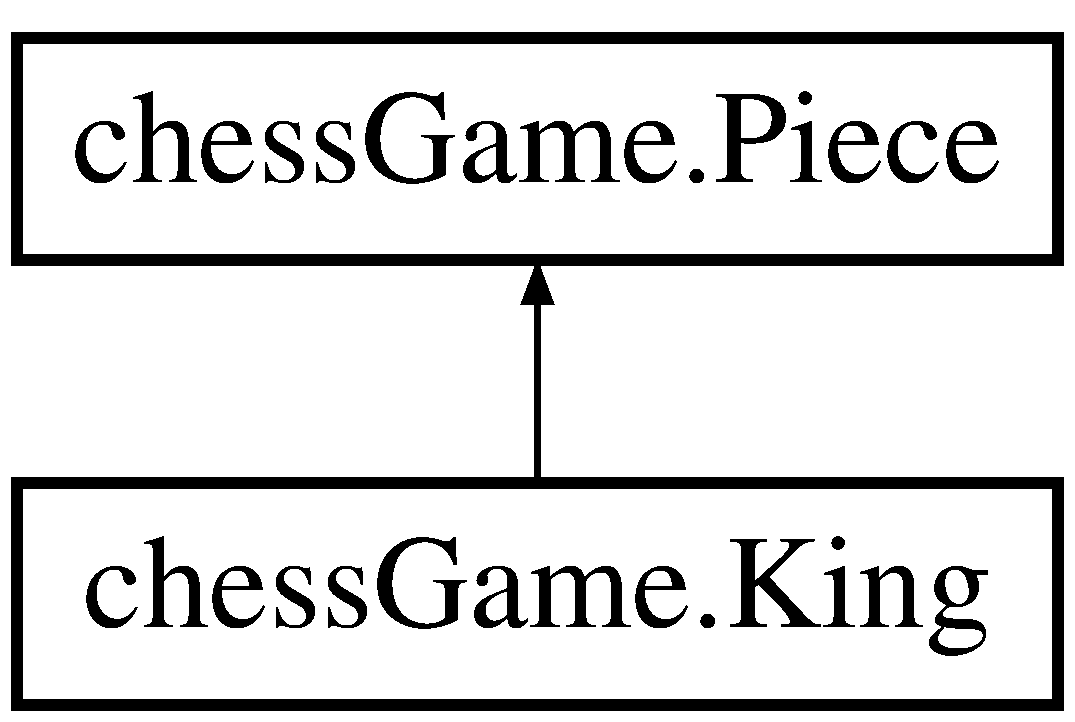
\includegraphics[height=2.000000cm]{classchess_game_1_1_king}
\end{center}
\end{figure}
\subsection*{Public Member Functions}
\begin{DoxyCompactItemize}
\item 
\hyperlink{classchess_game_1_1_king_a57fd36aaec2bb5284f32e28711d7d1e7}{King} (int \hyperlink{classchess_game_1_1_piece_aeb2d3374492005d799aa6b7b85be40e7}{x}, int \hyperlink{classchess_game_1_1_piece_a56e4d8d18eca3fd03a6bd5d6112d6359}{y}, \hyperlink{classchess_game_1_1_piece_ad5117cbbbaebf3a27c4f3c2bcbd6678b}{color} \hyperlink{classchess_game_1_1_piece_ad5117cbbbaebf3a27c4f3c2bcbd6678b}{color}, \hyperlink{classchess_game_1_1_piece_a1370c7f61581a1b72fa8ac2fd1af70a2}{type} \hyperlink{classchess_game_1_1_piece_a1370c7f61581a1b72fa8ac2fd1af70a2}{type})
\item 
boolean \hyperlink{classchess_game_1_1_king_a391861e09b20c62177db5f399ad94320}{check\+Destination} (int \hyperlink{classchess_game_1_1_piece_aeb2d3374492005d799aa6b7b85be40e7}{x}, int \hyperlink{classchess_game_1_1_piece_a56e4d8d18eca3fd03a6bd5d6112d6359}{y}, int turn, \hyperlink{classchess_game_1_1_chess_board}{Chess\+Board} board)
\end{DoxyCompactItemize}


\subsection{Constructor \& Destructor Documentation}
\hypertarget{classchess_game_1_1_king_a57fd36aaec2bb5284f32e28711d7d1e7}{}\label{classchess_game_1_1_king_a57fd36aaec2bb5284f32e28711d7d1e7} 
\index{chess\+Game\+::\+King@{chess\+Game\+::\+King}!King@{King}}
\index{King@{King}!chess\+Game\+::\+King@{chess\+Game\+::\+King}}
\subsubsection{\texorpdfstring{King()}{King()}}
{\footnotesize\ttfamily chess\+Game.\+King.\+King (\begin{DoxyParamCaption}\item[{int}]{x,  }\item[{int}]{y,  }\item[{\hyperlink{classchess_game_1_1_piece_ad5117cbbbaebf3a27c4f3c2bcbd6678b}{color}}]{color,  }\item[{\hyperlink{classchess_game_1_1_piece_a1370c7f61581a1b72fa8ac2fd1af70a2}{type}}]{type }\end{DoxyParamCaption})}



\subsection{Member Function Documentation}
\hypertarget{classchess_game_1_1_king_a391861e09b20c62177db5f399ad94320}{}\label{classchess_game_1_1_king_a391861e09b20c62177db5f399ad94320} 
\index{chess\+Game\+::\+King@{chess\+Game\+::\+King}!check\+Destination@{check\+Destination}}
\index{check\+Destination@{check\+Destination}!chess\+Game\+::\+King@{chess\+Game\+::\+King}}
\subsubsection{\texorpdfstring{check\+Destination()}{checkDestination()}}
{\footnotesize\ttfamily boolean chess\+Game.\+King.\+check\+Destination (\begin{DoxyParamCaption}\item[{int}]{x,  }\item[{int}]{y,  }\item[{int}]{turn,  }\item[{\hyperlink{classchess_game_1_1_chess_board}{Chess\+Board}}]{board }\end{DoxyParamCaption})}



The documentation for this class was generated from the following file\+:\begin{DoxyCompactItemize}
\item 
chess\+Game/\hyperlink{_king_8java}{King.\+java}\end{DoxyCompactItemize}

\hypertarget{classchess_game_1_1_knight}{}\section{chess\+Game.\+Knight Class Reference}
\label{classchess_game_1_1_knight}\index{chess\+Game.\+Knight@{chess\+Game.\+Knight}}
Inheritance diagram for chess\+Game.\+Knight\+:\begin{figure}[H]
\begin{center}
\leavevmode
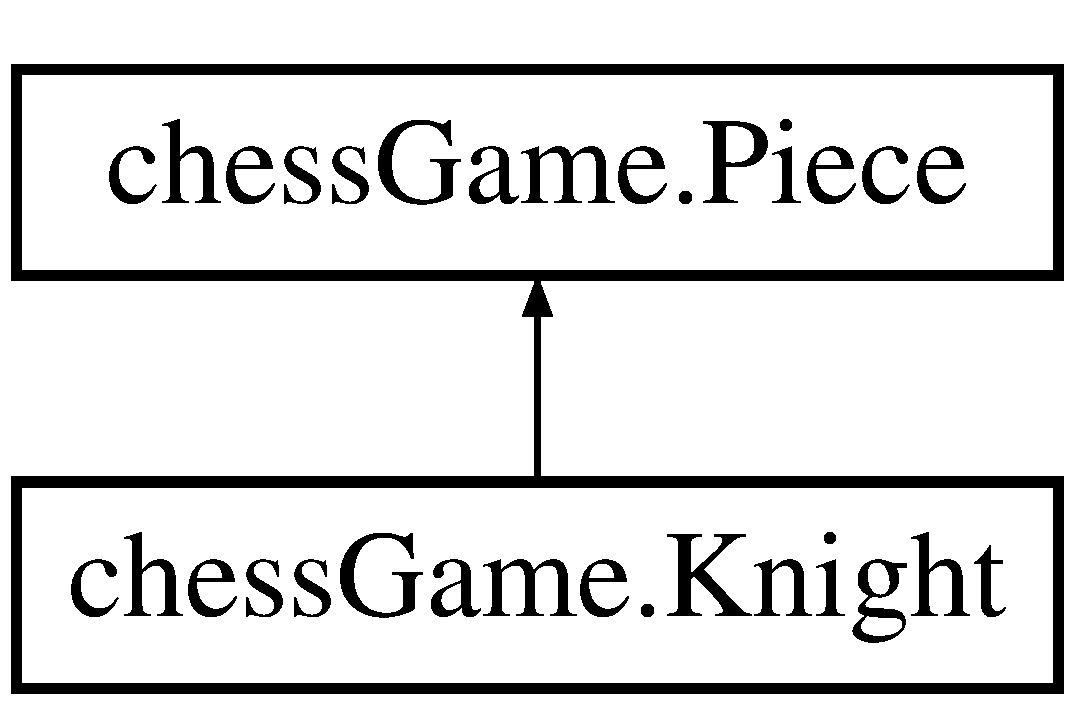
\includegraphics[height=2.000000cm]{classchess_game_1_1_knight}
\end{center}
\end{figure}
\subsection*{Public Member Functions}
\begin{DoxyCompactItemize}
\item 
\hyperlink{classchess_game_1_1_knight_a037b6cf54ad40d6e529bc5f92fbca382}{Knight} (int \hyperlink{classchess_game_1_1_piece_aeb2d3374492005d799aa6b7b85be40e7}{x}, int \hyperlink{classchess_game_1_1_piece_a56e4d8d18eca3fd03a6bd5d6112d6359}{y}, \hyperlink{classchess_game_1_1_piece_ad5117cbbbaebf3a27c4f3c2bcbd6678b}{color} \hyperlink{classchess_game_1_1_piece_ad5117cbbbaebf3a27c4f3c2bcbd6678b}{color}, \hyperlink{classchess_game_1_1_piece_a1370c7f61581a1b72fa8ac2fd1af70a2}{type} \hyperlink{classchess_game_1_1_piece_a1370c7f61581a1b72fa8ac2fd1af70a2}{type})
\item 
boolean \hyperlink{classchess_game_1_1_knight_a30cf3ee38afa826f026d39ac83ef15d8}{check\+Destination} (int \hyperlink{classchess_game_1_1_piece_aeb2d3374492005d799aa6b7b85be40e7}{x}, int \hyperlink{classchess_game_1_1_piece_a56e4d8d18eca3fd03a6bd5d6112d6359}{y}, int turn, \hyperlink{classchess_game_1_1_chess_board}{Chess\+Board} board)
\end{DoxyCompactItemize}


\subsection{Constructor \& Destructor Documentation}
\hypertarget{classchess_game_1_1_knight_a037b6cf54ad40d6e529bc5f92fbca382}{}\label{classchess_game_1_1_knight_a037b6cf54ad40d6e529bc5f92fbca382} 
\index{chess\+Game\+::\+Knight@{chess\+Game\+::\+Knight}!Knight@{Knight}}
\index{Knight@{Knight}!chess\+Game\+::\+Knight@{chess\+Game\+::\+Knight}}
\subsubsection{\texorpdfstring{Knight()}{Knight()}}
{\footnotesize\ttfamily chess\+Game.\+Knight.\+Knight (\begin{DoxyParamCaption}\item[{int}]{x,  }\item[{int}]{y,  }\item[{\hyperlink{classchess_game_1_1_piece_ad5117cbbbaebf3a27c4f3c2bcbd6678b}{color}}]{color,  }\item[{\hyperlink{classchess_game_1_1_piece_a1370c7f61581a1b72fa8ac2fd1af70a2}{type}}]{type }\end{DoxyParamCaption})}



\subsection{Member Function Documentation}
\hypertarget{classchess_game_1_1_knight_a30cf3ee38afa826f026d39ac83ef15d8}{}\label{classchess_game_1_1_knight_a30cf3ee38afa826f026d39ac83ef15d8} 
\index{chess\+Game\+::\+Knight@{chess\+Game\+::\+Knight}!check\+Destination@{check\+Destination}}
\index{check\+Destination@{check\+Destination}!chess\+Game\+::\+Knight@{chess\+Game\+::\+Knight}}
\subsubsection{\texorpdfstring{check\+Destination()}{checkDestination()}}
{\footnotesize\ttfamily boolean chess\+Game.\+Knight.\+check\+Destination (\begin{DoxyParamCaption}\item[{int}]{x,  }\item[{int}]{y,  }\item[{int}]{turn,  }\item[{\hyperlink{classchess_game_1_1_chess_board}{Chess\+Board}}]{board }\end{DoxyParamCaption})}



The documentation for this class was generated from the following file\+:\begin{DoxyCompactItemize}
\item 
chess\+Game/\hyperlink{_knight_8java}{Knight.\+java}\end{DoxyCompactItemize}

\hypertarget{classchess_game_1_1_pawn}{}\section{chess\+Game.\+Pawn Class Reference}
\label{classchess_game_1_1_pawn}\index{chess\+Game.\+Pawn@{chess\+Game.\+Pawn}}
Inheritance diagram for chess\+Game.\+Pawn\+:\begin{figure}[H]
\begin{center}
\leavevmode
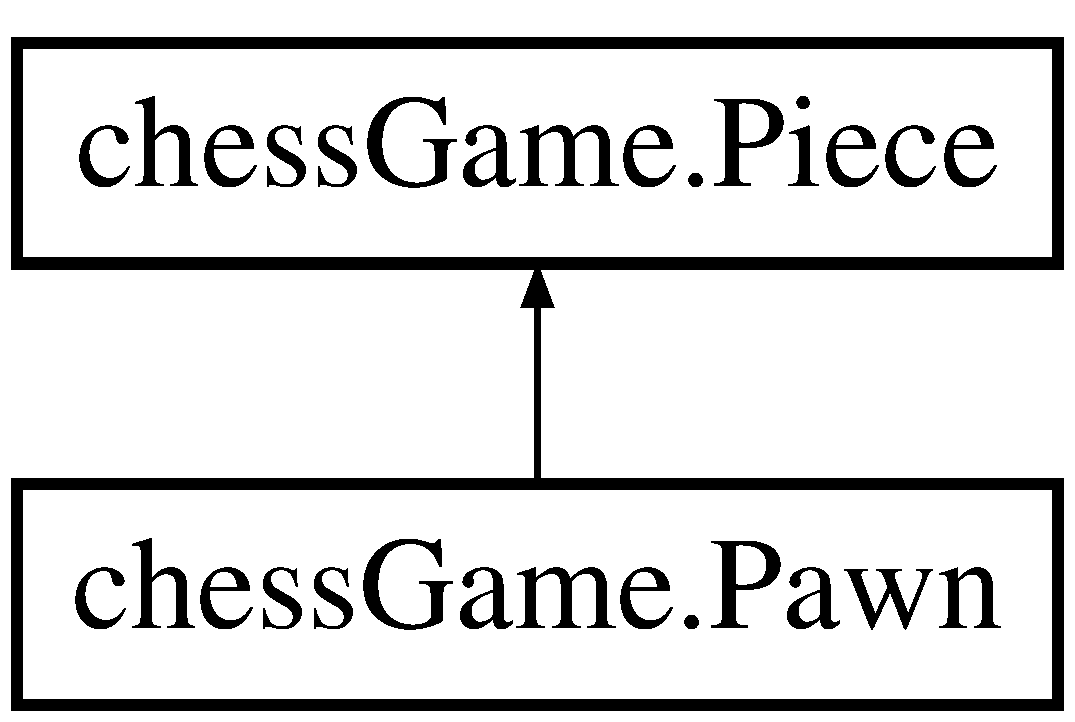
\includegraphics[height=2.000000cm]{classchess_game_1_1_pawn}
\end{center}
\end{figure}
\subsection*{Public Member Functions}
\begin{DoxyCompactItemize}
\item 
\hyperlink{classchess_game_1_1_pawn_a84303d22eb7d028cad8c5788dbf35581}{Pawn} (int \hyperlink{classchess_game_1_1_piece_aeb2d3374492005d799aa6b7b85be40e7}{x}, int \hyperlink{classchess_game_1_1_piece_a56e4d8d18eca3fd03a6bd5d6112d6359}{y}, \hyperlink{classchess_game_1_1_piece_ad5117cbbbaebf3a27c4f3c2bcbd6678b}{color} \hyperlink{classchess_game_1_1_piece_ad5117cbbbaebf3a27c4f3c2bcbd6678b}{color}, \hyperlink{classchess_game_1_1_piece_a1370c7f61581a1b72fa8ac2fd1af70a2}{type} \hyperlink{classchess_game_1_1_piece_a1370c7f61581a1b72fa8ac2fd1af70a2}{type})
\item 
boolean \hyperlink{classchess_game_1_1_pawn_ae85b0f679d8f19efc7d99c155633039f}{check\+Destination} (int \hyperlink{classchess_game_1_1_piece_aeb2d3374492005d799aa6b7b85be40e7}{x}, int \hyperlink{classchess_game_1_1_piece_a56e4d8d18eca3fd03a6bd5d6112d6359}{y}, int turn, \hyperlink{classchess_game_1_1_chess_board}{Chess\+Board} board)
\end{DoxyCompactItemize}


\subsection{Constructor \& Destructor Documentation}
\hypertarget{classchess_game_1_1_pawn_a84303d22eb7d028cad8c5788dbf35581}{}\label{classchess_game_1_1_pawn_a84303d22eb7d028cad8c5788dbf35581} 
\index{chess\+Game\+::\+Pawn@{chess\+Game\+::\+Pawn}!Pawn@{Pawn}}
\index{Pawn@{Pawn}!chess\+Game\+::\+Pawn@{chess\+Game\+::\+Pawn}}
\subsubsection{\texorpdfstring{Pawn()}{Pawn()}}
{\footnotesize\ttfamily chess\+Game.\+Pawn.\+Pawn (\begin{DoxyParamCaption}\item[{int}]{x,  }\item[{int}]{y,  }\item[{\hyperlink{classchess_game_1_1_piece_ad5117cbbbaebf3a27c4f3c2bcbd6678b}{color}}]{color,  }\item[{\hyperlink{classchess_game_1_1_piece_a1370c7f61581a1b72fa8ac2fd1af70a2}{type}}]{type }\end{DoxyParamCaption})}



\subsection{Member Function Documentation}
\hypertarget{classchess_game_1_1_pawn_ae85b0f679d8f19efc7d99c155633039f}{}\label{classchess_game_1_1_pawn_ae85b0f679d8f19efc7d99c155633039f} 
\index{chess\+Game\+::\+Pawn@{chess\+Game\+::\+Pawn}!check\+Destination@{check\+Destination}}
\index{check\+Destination@{check\+Destination}!chess\+Game\+::\+Pawn@{chess\+Game\+::\+Pawn}}
\subsubsection{\texorpdfstring{check\+Destination()}{checkDestination()}}
{\footnotesize\ttfamily boolean chess\+Game.\+Pawn.\+check\+Destination (\begin{DoxyParamCaption}\item[{int}]{x,  }\item[{int}]{y,  }\item[{int}]{turn,  }\item[{\hyperlink{classchess_game_1_1_chess_board}{Chess\+Board}}]{board }\end{DoxyParamCaption})}



The documentation for this class was generated from the following file\+:\begin{DoxyCompactItemize}
\item 
chess\+Game/\hyperlink{_pawn_8java}{Pawn.\+java}\end{DoxyCompactItemize}

\hypertarget{classchess_game_1_1_piece}{}\section{chess\+Game.\+Piece Class Reference}
\label{classchess_game_1_1_piece}\index{chess\+Game.\+Piece@{chess\+Game.\+Piece}}
Inheritance diagram for chess\+Game.\+Piece\+:\begin{figure}[H]
\begin{center}
\leavevmode
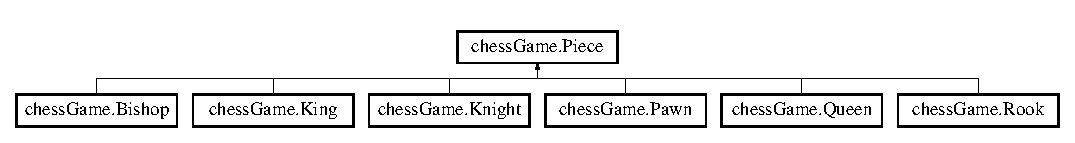
\includegraphics[height=1.469816cm]{classchess_game_1_1_piece}
\end{center}
\end{figure}
\subsection*{Classes}
\begin{DoxyCompactItemize}
\item 
enum {\bfseries color}
\item 
enum {\bfseries type}
\end{DoxyCompactItemize}
\subsection*{Public Member Functions}
\begin{DoxyCompactItemize}
\item 
\hyperlink{classchess_game_1_1_piece_ae619cd0f65a29cc3bd4c05cd0810f189}{Piece} (int \hyperlink{classchess_game_1_1_piece_aeb2d3374492005d799aa6b7b85be40e7}{x}, int \hyperlink{classchess_game_1_1_piece_a56e4d8d18eca3fd03a6bd5d6112d6359}{y}, \hyperlink{classchess_game_1_1_piece_ad5117cbbbaebf3a27c4f3c2bcbd6678b}{color} \hyperlink{classchess_game_1_1_piece_ad5117cbbbaebf3a27c4f3c2bcbd6678b}{color}, \hyperlink{classchess_game_1_1_piece_a1370c7f61581a1b72fa8ac2fd1af70a2}{type} \hyperlink{classchess_game_1_1_piece_a1370c7f61581a1b72fa8ac2fd1af70a2}{type})
\item 
int \hyperlink{classchess_game_1_1_piece_a7edc54b17ccd974a8039bfc701e4077a}{getX} ()
\item 
int \hyperlink{classchess_game_1_1_piece_acce32235b9e4d7aaf3a8459076b275e1}{getY} ()
\item 
\hyperlink{classchess_game_1_1_piece_ad5117cbbbaebf3a27c4f3c2bcbd6678b}{color} \hyperlink{classchess_game_1_1_piece_ad5b774ec1d029e20473344fe4669c589}{get\+Color} ()
\item 
boolean \hyperlink{classchess_game_1_1_piece_a1710ae14c4a78b3b3853c00be581132c}{get\+Alive} ()
\item 
\hyperlink{classchess_game_1_1_piece_a1370c7f61581a1b72fa8ac2fd1af70a2}{type} \hyperlink{classchess_game_1_1_piece_a057dfd4e48c07779e9d38b440785b2cc}{get\+Type} ()
\item 
void \hyperlink{classchess_game_1_1_piece_afb94aa7d6183aa2bb93d279dd3c5af35}{set\+Position} (int \hyperlink{classchess_game_1_1_piece_aeb2d3374492005d799aa6b7b85be40e7}{x}, int \hyperlink{classchess_game_1_1_piece_a56e4d8d18eca3fd03a6bd5d6112d6359}{y})
\item 
void \hyperlink{classchess_game_1_1_piece_a6dc59207045601b9efb024cd9ee4ccd4}{set\+Color} (\hyperlink{classchess_game_1_1_piece_ad5117cbbbaebf3a27c4f3c2bcbd6678b}{color} \hyperlink{classchess_game_1_1_piece_ad5117cbbbaebf3a27c4f3c2bcbd6678b}{color})
\item 
void \hyperlink{classchess_game_1_1_piece_af3f395afe64554bc7160c92981de2434}{set\+Alive} (boolean \hyperlink{classchess_game_1_1_piece_a887a90577f888865d9ec706397415026}{alive})
\item 
boolean \hyperlink{classchess_game_1_1_piece_ae4e70dd293be0d4fc4fb6b8e2e8f471f}{check\+Basics} (int \hyperlink{classchess_game_1_1_piece_aeb2d3374492005d799aa6b7b85be40e7}{x}, int \hyperlink{classchess_game_1_1_piece_a56e4d8d18eca3fd03a6bd5d6112d6359}{y}, int turn, \hyperlink{classchess_game_1_1_chess_board}{Chess\+Board} board)
\end{DoxyCompactItemize}
\subsection*{Private Attributes}
\begin{DoxyCompactItemize}
\item 
int \hyperlink{classchess_game_1_1_piece_aeb2d3374492005d799aa6b7b85be40e7}{x}
\item 
int \hyperlink{classchess_game_1_1_piece_a56e4d8d18eca3fd03a6bd5d6112d6359}{y}
\item 
boolean \hyperlink{classchess_game_1_1_piece_a887a90577f888865d9ec706397415026}{alive}
\item 
type \hyperlink{classchess_game_1_1_piece_a1370c7f61581a1b72fa8ac2fd1af70a2}{type}
\item 
color \hyperlink{classchess_game_1_1_piece_ad5117cbbbaebf3a27c4f3c2bcbd6678b}{color}
\end{DoxyCompactItemize}


\subsection{Constructor \& Destructor Documentation}
\hypertarget{classchess_game_1_1_piece_ae619cd0f65a29cc3bd4c05cd0810f189}{}\label{classchess_game_1_1_piece_ae619cd0f65a29cc3bd4c05cd0810f189} 
\index{chess\+Game\+::\+Piece@{chess\+Game\+::\+Piece}!Piece@{Piece}}
\index{Piece@{Piece}!chess\+Game\+::\+Piece@{chess\+Game\+::\+Piece}}
\subsubsection{\texorpdfstring{Piece()}{Piece()}}
{\footnotesize\ttfamily chess\+Game.\+Piece.\+Piece (\begin{DoxyParamCaption}\item[{int}]{x,  }\item[{int}]{y,  }\item[{\hyperlink{classchess_game_1_1_piece_ad5117cbbbaebf3a27c4f3c2bcbd6678b}{color}}]{color,  }\item[{\hyperlink{classchess_game_1_1_piece_a1370c7f61581a1b72fa8ac2fd1af70a2}{type}}]{type }\end{DoxyParamCaption})}



\subsection{Member Function Documentation}
\hypertarget{classchess_game_1_1_piece_ae4e70dd293be0d4fc4fb6b8e2e8f471f}{}\label{classchess_game_1_1_piece_ae4e70dd293be0d4fc4fb6b8e2e8f471f} 
\index{chess\+Game\+::\+Piece@{chess\+Game\+::\+Piece}!check\+Basics@{check\+Basics}}
\index{check\+Basics@{check\+Basics}!chess\+Game\+::\+Piece@{chess\+Game\+::\+Piece}}
\subsubsection{\texorpdfstring{check\+Basics()}{checkBasics()}}
{\footnotesize\ttfamily boolean chess\+Game.\+Piece.\+check\+Basics (\begin{DoxyParamCaption}\item[{int}]{x,  }\item[{int}]{y,  }\item[{int}]{turn,  }\item[{\hyperlink{classchess_game_1_1_chess_board}{Chess\+Board}}]{board }\end{DoxyParamCaption})}

\hypertarget{classchess_game_1_1_piece_a1710ae14c4a78b3b3853c00be581132c}{}\label{classchess_game_1_1_piece_a1710ae14c4a78b3b3853c00be581132c} 
\index{chess\+Game\+::\+Piece@{chess\+Game\+::\+Piece}!get\+Alive@{get\+Alive}}
\index{get\+Alive@{get\+Alive}!chess\+Game\+::\+Piece@{chess\+Game\+::\+Piece}}
\subsubsection{\texorpdfstring{get\+Alive()}{getAlive()}}
{\footnotesize\ttfamily boolean chess\+Game.\+Piece.\+get\+Alive (\begin{DoxyParamCaption}{ }\end{DoxyParamCaption})}

\hypertarget{classchess_game_1_1_piece_ad5b774ec1d029e20473344fe4669c589}{}\label{classchess_game_1_1_piece_ad5b774ec1d029e20473344fe4669c589} 
\index{chess\+Game\+::\+Piece@{chess\+Game\+::\+Piece}!get\+Color@{get\+Color}}
\index{get\+Color@{get\+Color}!chess\+Game\+::\+Piece@{chess\+Game\+::\+Piece}}
\subsubsection{\texorpdfstring{get\+Color()}{getColor()}}
{\footnotesize\ttfamily \hyperlink{classchess_game_1_1_piece_ad5117cbbbaebf3a27c4f3c2bcbd6678b}{color} chess\+Game.\+Piece.\+get\+Color (\begin{DoxyParamCaption}{ }\end{DoxyParamCaption})}

\hypertarget{classchess_game_1_1_piece_a057dfd4e48c07779e9d38b440785b2cc}{}\label{classchess_game_1_1_piece_a057dfd4e48c07779e9d38b440785b2cc} 
\index{chess\+Game\+::\+Piece@{chess\+Game\+::\+Piece}!get\+Type@{get\+Type}}
\index{get\+Type@{get\+Type}!chess\+Game\+::\+Piece@{chess\+Game\+::\+Piece}}
\subsubsection{\texorpdfstring{get\+Type()}{getType()}}
{\footnotesize\ttfamily \hyperlink{classchess_game_1_1_piece_a1370c7f61581a1b72fa8ac2fd1af70a2}{type} chess\+Game.\+Piece.\+get\+Type (\begin{DoxyParamCaption}{ }\end{DoxyParamCaption})}

\hypertarget{classchess_game_1_1_piece_a7edc54b17ccd974a8039bfc701e4077a}{}\label{classchess_game_1_1_piece_a7edc54b17ccd974a8039bfc701e4077a} 
\index{chess\+Game\+::\+Piece@{chess\+Game\+::\+Piece}!getX@{getX}}
\index{getX@{getX}!chess\+Game\+::\+Piece@{chess\+Game\+::\+Piece}}
\subsubsection{\texorpdfstring{get\+X()}{getX()}}
{\footnotesize\ttfamily int chess\+Game.\+Piece.\+getX (\begin{DoxyParamCaption}{ }\end{DoxyParamCaption})}

\hypertarget{classchess_game_1_1_piece_acce32235b9e4d7aaf3a8459076b275e1}{}\label{classchess_game_1_1_piece_acce32235b9e4d7aaf3a8459076b275e1} 
\index{chess\+Game\+::\+Piece@{chess\+Game\+::\+Piece}!getY@{getY}}
\index{getY@{getY}!chess\+Game\+::\+Piece@{chess\+Game\+::\+Piece}}
\subsubsection{\texorpdfstring{get\+Y()}{getY()}}
{\footnotesize\ttfamily int chess\+Game.\+Piece.\+getY (\begin{DoxyParamCaption}{ }\end{DoxyParamCaption})}

\hypertarget{classchess_game_1_1_piece_af3f395afe64554bc7160c92981de2434}{}\label{classchess_game_1_1_piece_af3f395afe64554bc7160c92981de2434} 
\index{chess\+Game\+::\+Piece@{chess\+Game\+::\+Piece}!set\+Alive@{set\+Alive}}
\index{set\+Alive@{set\+Alive}!chess\+Game\+::\+Piece@{chess\+Game\+::\+Piece}}
\subsubsection{\texorpdfstring{set\+Alive()}{setAlive()}}
{\footnotesize\ttfamily void chess\+Game.\+Piece.\+set\+Alive (\begin{DoxyParamCaption}\item[{boolean}]{alive }\end{DoxyParamCaption})}

\hypertarget{classchess_game_1_1_piece_a6dc59207045601b9efb024cd9ee4ccd4}{}\label{classchess_game_1_1_piece_a6dc59207045601b9efb024cd9ee4ccd4} 
\index{chess\+Game\+::\+Piece@{chess\+Game\+::\+Piece}!set\+Color@{set\+Color}}
\index{set\+Color@{set\+Color}!chess\+Game\+::\+Piece@{chess\+Game\+::\+Piece}}
\subsubsection{\texorpdfstring{set\+Color()}{setColor()}}
{\footnotesize\ttfamily void chess\+Game.\+Piece.\+set\+Color (\begin{DoxyParamCaption}\item[{\hyperlink{classchess_game_1_1_piece_ad5117cbbbaebf3a27c4f3c2bcbd6678b}{color}}]{color }\end{DoxyParamCaption})}

\hypertarget{classchess_game_1_1_piece_afb94aa7d6183aa2bb93d279dd3c5af35}{}\label{classchess_game_1_1_piece_afb94aa7d6183aa2bb93d279dd3c5af35} 
\index{chess\+Game\+::\+Piece@{chess\+Game\+::\+Piece}!set\+Position@{set\+Position}}
\index{set\+Position@{set\+Position}!chess\+Game\+::\+Piece@{chess\+Game\+::\+Piece}}
\subsubsection{\texorpdfstring{set\+Position()}{setPosition()}}
{\footnotesize\ttfamily void chess\+Game.\+Piece.\+set\+Position (\begin{DoxyParamCaption}\item[{int}]{x,  }\item[{int}]{y }\end{DoxyParamCaption})}



\subsection{Member Data Documentation}
\hypertarget{classchess_game_1_1_piece_a887a90577f888865d9ec706397415026}{}\label{classchess_game_1_1_piece_a887a90577f888865d9ec706397415026} 
\index{chess\+Game\+::\+Piece@{chess\+Game\+::\+Piece}!alive@{alive}}
\index{alive@{alive}!chess\+Game\+::\+Piece@{chess\+Game\+::\+Piece}}
\subsubsection{\texorpdfstring{alive}{alive}}
{\footnotesize\ttfamily boolean chess\+Game.\+Piece.\+alive\hspace{0.3cm}{\ttfamily [private]}}

\hypertarget{classchess_game_1_1_piece_ad5117cbbbaebf3a27c4f3c2bcbd6678b}{}\label{classchess_game_1_1_piece_ad5117cbbbaebf3a27c4f3c2bcbd6678b} 
\index{chess\+Game\+::\+Piece@{chess\+Game\+::\+Piece}!color@{color}}
\index{color@{color}!chess\+Game\+::\+Piece@{chess\+Game\+::\+Piece}}
\subsubsection{\texorpdfstring{color}{color}}
{\footnotesize\ttfamily color chess\+Game.\+Piece.\+color\hspace{0.3cm}{\ttfamily [private]}}

\hypertarget{classchess_game_1_1_piece_a1370c7f61581a1b72fa8ac2fd1af70a2}{}\label{classchess_game_1_1_piece_a1370c7f61581a1b72fa8ac2fd1af70a2} 
\index{chess\+Game\+::\+Piece@{chess\+Game\+::\+Piece}!type@{type}}
\index{type@{type}!chess\+Game\+::\+Piece@{chess\+Game\+::\+Piece}}
\subsubsection{\texorpdfstring{type}{type}}
{\footnotesize\ttfamily type chess\+Game.\+Piece.\+type\hspace{0.3cm}{\ttfamily [private]}}

\hypertarget{classchess_game_1_1_piece_aeb2d3374492005d799aa6b7b85be40e7}{}\label{classchess_game_1_1_piece_aeb2d3374492005d799aa6b7b85be40e7} 
\index{chess\+Game\+::\+Piece@{chess\+Game\+::\+Piece}!x@{x}}
\index{x@{x}!chess\+Game\+::\+Piece@{chess\+Game\+::\+Piece}}
\subsubsection{\texorpdfstring{x}{x}}
{\footnotesize\ttfamily int chess\+Game.\+Piece.\+x\hspace{0.3cm}{\ttfamily [private]}}

\hypertarget{classchess_game_1_1_piece_a56e4d8d18eca3fd03a6bd5d6112d6359}{}\label{classchess_game_1_1_piece_a56e4d8d18eca3fd03a6bd5d6112d6359} 
\index{chess\+Game\+::\+Piece@{chess\+Game\+::\+Piece}!y@{y}}
\index{y@{y}!chess\+Game\+::\+Piece@{chess\+Game\+::\+Piece}}
\subsubsection{\texorpdfstring{y}{y}}
{\footnotesize\ttfamily int chess\+Game.\+Piece.\+y\hspace{0.3cm}{\ttfamily [private]}}



The documentation for this class was generated from the following file\+:\begin{DoxyCompactItemize}
\item 
chess\+Game/\hyperlink{_piece_8java}{Piece.\+java}\end{DoxyCompactItemize}

\hypertarget{classchess_game_1_1_queen}{}\section{chess\+Game.\+Queen Class Reference}
\label{classchess_game_1_1_queen}\index{chess\+Game.\+Queen@{chess\+Game.\+Queen}}
Inheritance diagram for chess\+Game.\+Queen\+:\begin{figure}[H]
\begin{center}
\leavevmode
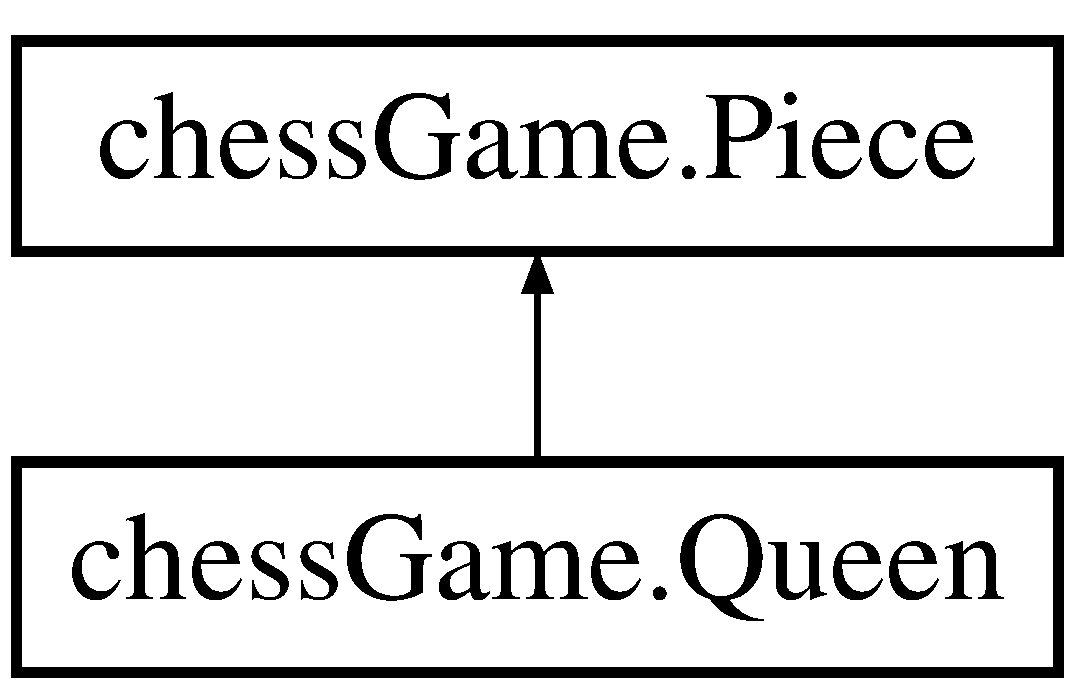
\includegraphics[height=2.000000cm]{classchess_game_1_1_queen}
\end{center}
\end{figure}
\subsection*{Public Member Functions}
\begin{DoxyCompactItemize}
\item 
\hyperlink{classchess_game_1_1_queen_add4682e5e02e4a89a518c4f12eae9346}{Queen} (int \hyperlink{classchess_game_1_1_piece_aeb2d3374492005d799aa6b7b85be40e7}{x}, int \hyperlink{classchess_game_1_1_piece_a56e4d8d18eca3fd03a6bd5d6112d6359}{y}, \hyperlink{classchess_game_1_1_piece_ad5117cbbbaebf3a27c4f3c2bcbd6678b}{color} \hyperlink{classchess_game_1_1_piece_ad5117cbbbaebf3a27c4f3c2bcbd6678b}{color}, \hyperlink{classchess_game_1_1_piece_a1370c7f61581a1b72fa8ac2fd1af70a2}{type} \hyperlink{classchess_game_1_1_piece_a1370c7f61581a1b72fa8ac2fd1af70a2}{type})
\item 
boolean \hyperlink{classchess_game_1_1_queen_af27e38067888a18cb60dc3f9f7e2a87c}{check\+Destination} (int \hyperlink{classchess_game_1_1_piece_aeb2d3374492005d799aa6b7b85be40e7}{x}, int \hyperlink{classchess_game_1_1_piece_a56e4d8d18eca3fd03a6bd5d6112d6359}{y}, int turn, \hyperlink{classchess_game_1_1_chess_board}{Chess\+Board} board)
\end{DoxyCompactItemize}


\subsection{Constructor \& Destructor Documentation}
\hypertarget{classchess_game_1_1_queen_add4682e5e02e4a89a518c4f12eae9346}{}\label{classchess_game_1_1_queen_add4682e5e02e4a89a518c4f12eae9346} 
\index{chess\+Game\+::\+Queen@{chess\+Game\+::\+Queen}!Queen@{Queen}}
\index{Queen@{Queen}!chess\+Game\+::\+Queen@{chess\+Game\+::\+Queen}}
\subsubsection{\texorpdfstring{Queen()}{Queen()}}
{\footnotesize\ttfamily chess\+Game.\+Queen.\+Queen (\begin{DoxyParamCaption}\item[{int}]{x,  }\item[{int}]{y,  }\item[{\hyperlink{classchess_game_1_1_piece_ad5117cbbbaebf3a27c4f3c2bcbd6678b}{color}}]{color,  }\item[{\hyperlink{classchess_game_1_1_piece_a1370c7f61581a1b72fa8ac2fd1af70a2}{type}}]{type }\end{DoxyParamCaption})}



\subsection{Member Function Documentation}
\hypertarget{classchess_game_1_1_queen_af27e38067888a18cb60dc3f9f7e2a87c}{}\label{classchess_game_1_1_queen_af27e38067888a18cb60dc3f9f7e2a87c} 
\index{chess\+Game\+::\+Queen@{chess\+Game\+::\+Queen}!check\+Destination@{check\+Destination}}
\index{check\+Destination@{check\+Destination}!chess\+Game\+::\+Queen@{chess\+Game\+::\+Queen}}
\subsubsection{\texorpdfstring{check\+Destination()}{checkDestination()}}
{\footnotesize\ttfamily boolean chess\+Game.\+Queen.\+check\+Destination (\begin{DoxyParamCaption}\item[{int}]{x,  }\item[{int}]{y,  }\item[{int}]{turn,  }\item[{\hyperlink{classchess_game_1_1_chess_board}{Chess\+Board}}]{board }\end{DoxyParamCaption})}



The documentation for this class was generated from the following file\+:\begin{DoxyCompactItemize}
\item 
chess\+Game/\hyperlink{_queen_8java}{Queen.\+java}\end{DoxyCompactItemize}

\hypertarget{classchess_game_1_1_rook}{}\section{chess\+Game.\+Rook Class Reference}
\label{classchess_game_1_1_rook}\index{chess\+Game.\+Rook@{chess\+Game.\+Rook}}
Inheritance diagram for chess\+Game.\+Rook\+:\begin{figure}[H]
\begin{center}
\leavevmode
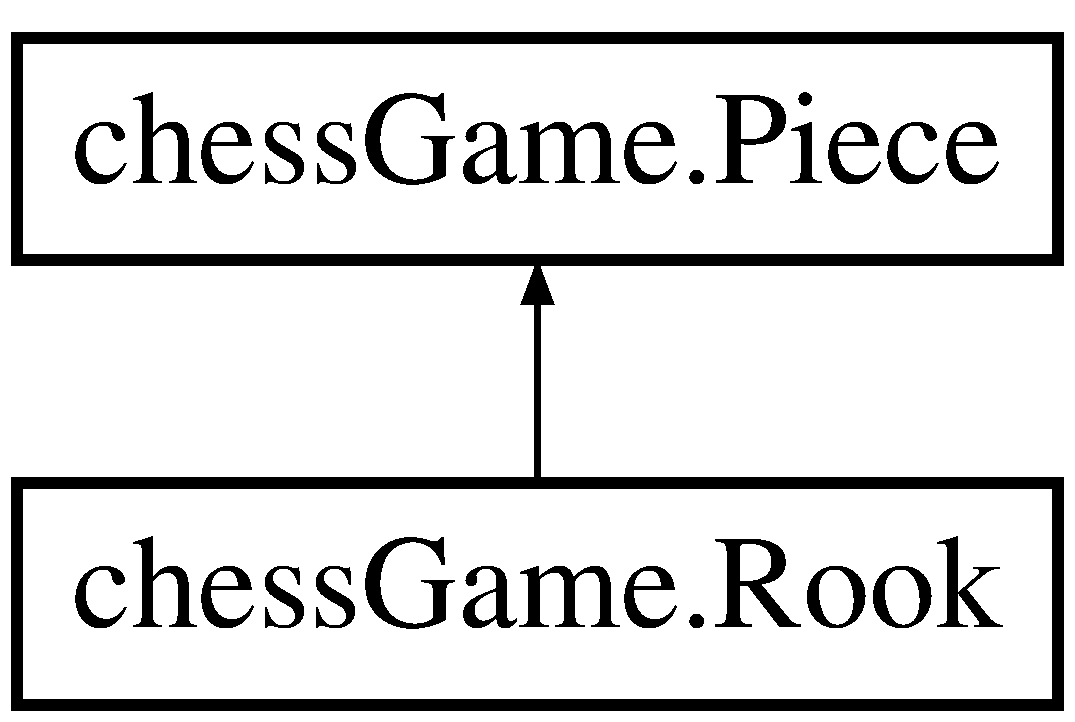
\includegraphics[height=2.000000cm]{classchess_game_1_1_rook}
\end{center}
\end{figure}
\subsection*{Public Member Functions}
\begin{DoxyCompactItemize}
\item 
\hyperlink{classchess_game_1_1_rook_ab18090f0e1c42f60f3e0a89fdf599843}{Rook} (int \hyperlink{classchess_game_1_1_piece_aeb2d3374492005d799aa6b7b85be40e7}{x}, int \hyperlink{classchess_game_1_1_piece_a56e4d8d18eca3fd03a6bd5d6112d6359}{y}, \hyperlink{classchess_game_1_1_piece_ad5117cbbbaebf3a27c4f3c2bcbd6678b}{color} \hyperlink{classchess_game_1_1_piece_ad5117cbbbaebf3a27c4f3c2bcbd6678b}{color}, \hyperlink{classchess_game_1_1_piece_a1370c7f61581a1b72fa8ac2fd1af70a2}{type} \hyperlink{classchess_game_1_1_piece_a1370c7f61581a1b72fa8ac2fd1af70a2}{type})
\item 
boolean \hyperlink{classchess_game_1_1_rook_a8b9521d22b59e973c8bbd1e36dd70977}{check\+Destination} (int \hyperlink{classchess_game_1_1_piece_aeb2d3374492005d799aa6b7b85be40e7}{x}, int \hyperlink{classchess_game_1_1_piece_a56e4d8d18eca3fd03a6bd5d6112d6359}{y}, int turn, \hyperlink{classchess_game_1_1_chess_board}{Chess\+Board} board)
\end{DoxyCompactItemize}


\subsection{Constructor \& Destructor Documentation}
\hypertarget{classchess_game_1_1_rook_ab18090f0e1c42f60f3e0a89fdf599843}{}\label{classchess_game_1_1_rook_ab18090f0e1c42f60f3e0a89fdf599843} 
\index{chess\+Game\+::\+Rook@{chess\+Game\+::\+Rook}!Rook@{Rook}}
\index{Rook@{Rook}!chess\+Game\+::\+Rook@{chess\+Game\+::\+Rook}}
\subsubsection{\texorpdfstring{Rook()}{Rook()}}
{\footnotesize\ttfamily chess\+Game.\+Rook.\+Rook (\begin{DoxyParamCaption}\item[{int}]{x,  }\item[{int}]{y,  }\item[{\hyperlink{classchess_game_1_1_piece_ad5117cbbbaebf3a27c4f3c2bcbd6678b}{color}}]{color,  }\item[{\hyperlink{classchess_game_1_1_piece_a1370c7f61581a1b72fa8ac2fd1af70a2}{type}}]{type }\end{DoxyParamCaption})}



\subsection{Member Function Documentation}
\hypertarget{classchess_game_1_1_rook_a8b9521d22b59e973c8bbd1e36dd70977}{}\label{classchess_game_1_1_rook_a8b9521d22b59e973c8bbd1e36dd70977} 
\index{chess\+Game\+::\+Rook@{chess\+Game\+::\+Rook}!check\+Destination@{check\+Destination}}
\index{check\+Destination@{check\+Destination}!chess\+Game\+::\+Rook@{chess\+Game\+::\+Rook}}
\subsubsection{\texorpdfstring{check\+Destination()}{checkDestination()}}
{\footnotesize\ttfamily boolean chess\+Game.\+Rook.\+check\+Destination (\begin{DoxyParamCaption}\item[{int}]{x,  }\item[{int}]{y,  }\item[{int}]{turn,  }\item[{\hyperlink{classchess_game_1_1_chess_board}{Chess\+Board}}]{board }\end{DoxyParamCaption})}



The documentation for this class was generated from the following file\+:\begin{DoxyCompactItemize}
\item 
chess\+Game/\hyperlink{_rook_8java}{Rook.\+java}\end{DoxyCompactItemize}

\hypertarget{classchess_game_1_1_tests_one}{}\section{chess\+Game.\+Tests\+One Class Reference}
\label{classchess_game_1_1_tests_one}\index{chess\+Game.\+Tests\+One@{chess\+Game.\+Tests\+One}}
\subsection*{Public Member Functions}
\begin{DoxyCompactItemize}
\item 
void \hyperlink{classchess_game_1_1_tests_one_a5ad1d4e10e2d9f7dd68ab8e1f98d30df}{test\+Board\+White} ()
\item 
void \hyperlink{classchess_game_1_1_tests_one_aa5af1f8650fba37708180074d50f9d12}{test\+Board\+Black} ()
\item 
void \hyperlink{classchess_game_1_1_tests_one_aea568b72ac003ecc7b6aef884c11ba1e}{test\+Selection\+Good} ()
\item 
void \hyperlink{classchess_game_1_1_tests_one_ac7e3b12d75a0134942a6d1b78cf93e6d}{test\+Selection\+Bad} ()
\item 
void \hyperlink{classchess_game_1_1_tests_one_a8fe235e622e35e564c11266c662aa1eb}{test\+Make\+Move} ()
\item 
void \hyperlink{classchess_game_1_1_tests_one_a761a9c74c24b69d572b83dc985ac0983}{check\+Destination\+Pawn\+Good} ()
\item 
void \hyperlink{classchess_game_1_1_tests_one_a5574aa9835757dbe5a9475e6dc299363}{check\+Destination\+Pawn\+Bad} ()
\item 
void \hyperlink{classchess_game_1_1_tests_one_aa9306477b5a3dcda3a5fcdf26cae704e}{check\+Destination\+Rook\+Good} ()
\item 
void \hyperlink{classchess_game_1_1_tests_one_a3a084e7f8ae5961032e344dc0971a30c}{check\+Destination\+Rook\+Bad} ()
\item 
void \hyperlink{classchess_game_1_1_tests_one_a433f857badf4ba90f5689af141834f2a}{check\+Destination\+Knight\+Good} ()
\item 
void \hyperlink{classchess_game_1_1_tests_one_abad959a4f06760f812cf016ea0f1c756}{check\+Destination\+Knight\+Bad} ()
\item 
void \hyperlink{classchess_game_1_1_tests_one_a8b2708dd6b64dbfc7387ba22844c9e9f}{check\+Destination\+Bishop\+Good} ()
\item 
void \hyperlink{classchess_game_1_1_tests_one_a4bac71560076146506952017cbe45a3f}{check\+Destination\+Bishop\+Bad} ()
\item 
void \hyperlink{classchess_game_1_1_tests_one_af3bc1e11e160379dd884aa09ebb6d5b4}{check\+Destination\+Queen\+Good} ()
\item 
void \hyperlink{classchess_game_1_1_tests_one_a0c41ad0a4b9fe727288eb67f82065d6b}{check\+Destination\+Queen\+Bad} ()
\item 
void \hyperlink{classchess_game_1_1_tests_one_a256844b22f9f1d9137a49a72d1847fce}{check\+Destination\+King\+Good} ()
\item 
void \hyperlink{classchess_game_1_1_tests_one_aa2659eaaf952de90d827cb12b0e7c0e2}{check\+Destination\+King\+Bad} ()
\end{DoxyCompactItemize}


\subsection{Member Function Documentation}
\hypertarget{classchess_game_1_1_tests_one_a4bac71560076146506952017cbe45a3f}{}\label{classchess_game_1_1_tests_one_a4bac71560076146506952017cbe45a3f} 
\index{chess\+Game\+::\+Tests\+One@{chess\+Game\+::\+Tests\+One}!check\+Destination\+Bishop\+Bad@{check\+Destination\+Bishop\+Bad}}
\index{check\+Destination\+Bishop\+Bad@{check\+Destination\+Bishop\+Bad}!chess\+Game\+::\+Tests\+One@{chess\+Game\+::\+Tests\+One}}
\subsubsection{\texorpdfstring{check\+Destination\+Bishop\+Bad()}{checkDestinationBishopBad()}}
{\footnotesize\ttfamily void chess\+Game.\+Tests\+One.\+check\+Destination\+Bishop\+Bad (\begin{DoxyParamCaption}{ }\end{DoxyParamCaption})}

\hypertarget{classchess_game_1_1_tests_one_a8b2708dd6b64dbfc7387ba22844c9e9f}{}\label{classchess_game_1_1_tests_one_a8b2708dd6b64dbfc7387ba22844c9e9f} 
\index{chess\+Game\+::\+Tests\+One@{chess\+Game\+::\+Tests\+One}!check\+Destination\+Bishop\+Good@{check\+Destination\+Bishop\+Good}}
\index{check\+Destination\+Bishop\+Good@{check\+Destination\+Bishop\+Good}!chess\+Game\+::\+Tests\+One@{chess\+Game\+::\+Tests\+One}}
\subsubsection{\texorpdfstring{check\+Destination\+Bishop\+Good()}{checkDestinationBishopGood()}}
{\footnotesize\ttfamily void chess\+Game.\+Tests\+One.\+check\+Destination\+Bishop\+Good (\begin{DoxyParamCaption}{ }\end{DoxyParamCaption})}

\hypertarget{classchess_game_1_1_tests_one_aa2659eaaf952de90d827cb12b0e7c0e2}{}\label{classchess_game_1_1_tests_one_aa2659eaaf952de90d827cb12b0e7c0e2} 
\index{chess\+Game\+::\+Tests\+One@{chess\+Game\+::\+Tests\+One}!check\+Destination\+King\+Bad@{check\+Destination\+King\+Bad}}
\index{check\+Destination\+King\+Bad@{check\+Destination\+King\+Bad}!chess\+Game\+::\+Tests\+One@{chess\+Game\+::\+Tests\+One}}
\subsubsection{\texorpdfstring{check\+Destination\+King\+Bad()}{checkDestinationKingBad()}}
{\footnotesize\ttfamily void chess\+Game.\+Tests\+One.\+check\+Destination\+King\+Bad (\begin{DoxyParamCaption}{ }\end{DoxyParamCaption})}

\hypertarget{classchess_game_1_1_tests_one_a256844b22f9f1d9137a49a72d1847fce}{}\label{classchess_game_1_1_tests_one_a256844b22f9f1d9137a49a72d1847fce} 
\index{chess\+Game\+::\+Tests\+One@{chess\+Game\+::\+Tests\+One}!check\+Destination\+King\+Good@{check\+Destination\+King\+Good}}
\index{check\+Destination\+King\+Good@{check\+Destination\+King\+Good}!chess\+Game\+::\+Tests\+One@{chess\+Game\+::\+Tests\+One}}
\subsubsection{\texorpdfstring{check\+Destination\+King\+Good()}{checkDestinationKingGood()}}
{\footnotesize\ttfamily void chess\+Game.\+Tests\+One.\+check\+Destination\+King\+Good (\begin{DoxyParamCaption}{ }\end{DoxyParamCaption})}

\hypertarget{classchess_game_1_1_tests_one_abad959a4f06760f812cf016ea0f1c756}{}\label{classchess_game_1_1_tests_one_abad959a4f06760f812cf016ea0f1c756} 
\index{chess\+Game\+::\+Tests\+One@{chess\+Game\+::\+Tests\+One}!check\+Destination\+Knight\+Bad@{check\+Destination\+Knight\+Bad}}
\index{check\+Destination\+Knight\+Bad@{check\+Destination\+Knight\+Bad}!chess\+Game\+::\+Tests\+One@{chess\+Game\+::\+Tests\+One}}
\subsubsection{\texorpdfstring{check\+Destination\+Knight\+Bad()}{checkDestinationKnightBad()}}
{\footnotesize\ttfamily void chess\+Game.\+Tests\+One.\+check\+Destination\+Knight\+Bad (\begin{DoxyParamCaption}{ }\end{DoxyParamCaption})}

\hypertarget{classchess_game_1_1_tests_one_a433f857badf4ba90f5689af141834f2a}{}\label{classchess_game_1_1_tests_one_a433f857badf4ba90f5689af141834f2a} 
\index{chess\+Game\+::\+Tests\+One@{chess\+Game\+::\+Tests\+One}!check\+Destination\+Knight\+Good@{check\+Destination\+Knight\+Good}}
\index{check\+Destination\+Knight\+Good@{check\+Destination\+Knight\+Good}!chess\+Game\+::\+Tests\+One@{chess\+Game\+::\+Tests\+One}}
\subsubsection{\texorpdfstring{check\+Destination\+Knight\+Good()}{checkDestinationKnightGood()}}
{\footnotesize\ttfamily void chess\+Game.\+Tests\+One.\+check\+Destination\+Knight\+Good (\begin{DoxyParamCaption}{ }\end{DoxyParamCaption})}

\hypertarget{classchess_game_1_1_tests_one_a5574aa9835757dbe5a9475e6dc299363}{}\label{classchess_game_1_1_tests_one_a5574aa9835757dbe5a9475e6dc299363} 
\index{chess\+Game\+::\+Tests\+One@{chess\+Game\+::\+Tests\+One}!check\+Destination\+Pawn\+Bad@{check\+Destination\+Pawn\+Bad}}
\index{check\+Destination\+Pawn\+Bad@{check\+Destination\+Pawn\+Bad}!chess\+Game\+::\+Tests\+One@{chess\+Game\+::\+Tests\+One}}
\subsubsection{\texorpdfstring{check\+Destination\+Pawn\+Bad()}{checkDestinationPawnBad()}}
{\footnotesize\ttfamily void chess\+Game.\+Tests\+One.\+check\+Destination\+Pawn\+Bad (\begin{DoxyParamCaption}{ }\end{DoxyParamCaption})}

\hypertarget{classchess_game_1_1_tests_one_a761a9c74c24b69d572b83dc985ac0983}{}\label{classchess_game_1_1_tests_one_a761a9c74c24b69d572b83dc985ac0983} 
\index{chess\+Game\+::\+Tests\+One@{chess\+Game\+::\+Tests\+One}!check\+Destination\+Pawn\+Good@{check\+Destination\+Pawn\+Good}}
\index{check\+Destination\+Pawn\+Good@{check\+Destination\+Pawn\+Good}!chess\+Game\+::\+Tests\+One@{chess\+Game\+::\+Tests\+One}}
\subsubsection{\texorpdfstring{check\+Destination\+Pawn\+Good()}{checkDestinationPawnGood()}}
{\footnotesize\ttfamily void chess\+Game.\+Tests\+One.\+check\+Destination\+Pawn\+Good (\begin{DoxyParamCaption}{ }\end{DoxyParamCaption})}

\hypertarget{classchess_game_1_1_tests_one_a0c41ad0a4b9fe727288eb67f82065d6b}{}\label{classchess_game_1_1_tests_one_a0c41ad0a4b9fe727288eb67f82065d6b} 
\index{chess\+Game\+::\+Tests\+One@{chess\+Game\+::\+Tests\+One}!check\+Destination\+Queen\+Bad@{check\+Destination\+Queen\+Bad}}
\index{check\+Destination\+Queen\+Bad@{check\+Destination\+Queen\+Bad}!chess\+Game\+::\+Tests\+One@{chess\+Game\+::\+Tests\+One}}
\subsubsection{\texorpdfstring{check\+Destination\+Queen\+Bad()}{checkDestinationQueenBad()}}
{\footnotesize\ttfamily void chess\+Game.\+Tests\+One.\+check\+Destination\+Queen\+Bad (\begin{DoxyParamCaption}{ }\end{DoxyParamCaption})}

\hypertarget{classchess_game_1_1_tests_one_af3bc1e11e160379dd884aa09ebb6d5b4}{}\label{classchess_game_1_1_tests_one_af3bc1e11e160379dd884aa09ebb6d5b4} 
\index{chess\+Game\+::\+Tests\+One@{chess\+Game\+::\+Tests\+One}!check\+Destination\+Queen\+Good@{check\+Destination\+Queen\+Good}}
\index{check\+Destination\+Queen\+Good@{check\+Destination\+Queen\+Good}!chess\+Game\+::\+Tests\+One@{chess\+Game\+::\+Tests\+One}}
\subsubsection{\texorpdfstring{check\+Destination\+Queen\+Good()}{checkDestinationQueenGood()}}
{\footnotesize\ttfamily void chess\+Game.\+Tests\+One.\+check\+Destination\+Queen\+Good (\begin{DoxyParamCaption}{ }\end{DoxyParamCaption})}

\hypertarget{classchess_game_1_1_tests_one_a3a084e7f8ae5961032e344dc0971a30c}{}\label{classchess_game_1_1_tests_one_a3a084e7f8ae5961032e344dc0971a30c} 
\index{chess\+Game\+::\+Tests\+One@{chess\+Game\+::\+Tests\+One}!check\+Destination\+Rook\+Bad@{check\+Destination\+Rook\+Bad}}
\index{check\+Destination\+Rook\+Bad@{check\+Destination\+Rook\+Bad}!chess\+Game\+::\+Tests\+One@{chess\+Game\+::\+Tests\+One}}
\subsubsection{\texorpdfstring{check\+Destination\+Rook\+Bad()}{checkDestinationRookBad()}}
{\footnotesize\ttfamily void chess\+Game.\+Tests\+One.\+check\+Destination\+Rook\+Bad (\begin{DoxyParamCaption}{ }\end{DoxyParamCaption})}

\hypertarget{classchess_game_1_1_tests_one_aa9306477b5a3dcda3a5fcdf26cae704e}{}\label{classchess_game_1_1_tests_one_aa9306477b5a3dcda3a5fcdf26cae704e} 
\index{chess\+Game\+::\+Tests\+One@{chess\+Game\+::\+Tests\+One}!check\+Destination\+Rook\+Good@{check\+Destination\+Rook\+Good}}
\index{check\+Destination\+Rook\+Good@{check\+Destination\+Rook\+Good}!chess\+Game\+::\+Tests\+One@{chess\+Game\+::\+Tests\+One}}
\subsubsection{\texorpdfstring{check\+Destination\+Rook\+Good()}{checkDestinationRookGood()}}
{\footnotesize\ttfamily void chess\+Game.\+Tests\+One.\+check\+Destination\+Rook\+Good (\begin{DoxyParamCaption}{ }\end{DoxyParamCaption})}

\hypertarget{classchess_game_1_1_tests_one_aa5af1f8650fba37708180074d50f9d12}{}\label{classchess_game_1_1_tests_one_aa5af1f8650fba37708180074d50f9d12} 
\index{chess\+Game\+::\+Tests\+One@{chess\+Game\+::\+Tests\+One}!test\+Board\+Black@{test\+Board\+Black}}
\index{test\+Board\+Black@{test\+Board\+Black}!chess\+Game\+::\+Tests\+One@{chess\+Game\+::\+Tests\+One}}
\subsubsection{\texorpdfstring{test\+Board\+Black()}{testBoardBlack()}}
{\footnotesize\ttfamily void chess\+Game.\+Tests\+One.\+test\+Board\+Black (\begin{DoxyParamCaption}{ }\end{DoxyParamCaption})}

\hypertarget{classchess_game_1_1_tests_one_a5ad1d4e10e2d9f7dd68ab8e1f98d30df}{}\label{classchess_game_1_1_tests_one_a5ad1d4e10e2d9f7dd68ab8e1f98d30df} 
\index{chess\+Game\+::\+Tests\+One@{chess\+Game\+::\+Tests\+One}!test\+Board\+White@{test\+Board\+White}}
\index{test\+Board\+White@{test\+Board\+White}!chess\+Game\+::\+Tests\+One@{chess\+Game\+::\+Tests\+One}}
\subsubsection{\texorpdfstring{test\+Board\+White()}{testBoardWhite()}}
{\footnotesize\ttfamily void chess\+Game.\+Tests\+One.\+test\+Board\+White (\begin{DoxyParamCaption}{ }\end{DoxyParamCaption})}

\hypertarget{classchess_game_1_1_tests_one_a8fe235e622e35e564c11266c662aa1eb}{}\label{classchess_game_1_1_tests_one_a8fe235e622e35e564c11266c662aa1eb} 
\index{chess\+Game\+::\+Tests\+One@{chess\+Game\+::\+Tests\+One}!test\+Make\+Move@{test\+Make\+Move}}
\index{test\+Make\+Move@{test\+Make\+Move}!chess\+Game\+::\+Tests\+One@{chess\+Game\+::\+Tests\+One}}
\subsubsection{\texorpdfstring{test\+Make\+Move()}{testMakeMove()}}
{\footnotesize\ttfamily void chess\+Game.\+Tests\+One.\+test\+Make\+Move (\begin{DoxyParamCaption}{ }\end{DoxyParamCaption})}

\hypertarget{classchess_game_1_1_tests_one_ac7e3b12d75a0134942a6d1b78cf93e6d}{}\label{classchess_game_1_1_tests_one_ac7e3b12d75a0134942a6d1b78cf93e6d} 
\index{chess\+Game\+::\+Tests\+One@{chess\+Game\+::\+Tests\+One}!test\+Selection\+Bad@{test\+Selection\+Bad}}
\index{test\+Selection\+Bad@{test\+Selection\+Bad}!chess\+Game\+::\+Tests\+One@{chess\+Game\+::\+Tests\+One}}
\subsubsection{\texorpdfstring{test\+Selection\+Bad()}{testSelectionBad()}}
{\footnotesize\ttfamily void chess\+Game.\+Tests\+One.\+test\+Selection\+Bad (\begin{DoxyParamCaption}{ }\end{DoxyParamCaption})}

\hypertarget{classchess_game_1_1_tests_one_aea568b72ac003ecc7b6aef884c11ba1e}{}\label{classchess_game_1_1_tests_one_aea568b72ac003ecc7b6aef884c11ba1e} 
\index{chess\+Game\+::\+Tests\+One@{chess\+Game\+::\+Tests\+One}!test\+Selection\+Good@{test\+Selection\+Good}}
\index{test\+Selection\+Good@{test\+Selection\+Good}!chess\+Game\+::\+Tests\+One@{chess\+Game\+::\+Tests\+One}}
\subsubsection{\texorpdfstring{test\+Selection\+Good()}{testSelectionGood()}}
{\footnotesize\ttfamily void chess\+Game.\+Tests\+One.\+test\+Selection\+Good (\begin{DoxyParamCaption}{ }\end{DoxyParamCaption})}



The documentation for this class was generated from the following file\+:\begin{DoxyCompactItemize}
\item 
chess\+Game/\hyperlink{_tests_one_8java}{Tests\+One.\+java}\end{DoxyCompactItemize}

\chapter{File Documentation}
\hypertarget{_bishop_8java}{}\section{chess\+Game/\+Bishop.java File Reference}
\label{_bishop_8java}\index{chess\+Game/\+Bishop.\+java@{chess\+Game/\+Bishop.\+java}}
\subsection*{Classes}
\begin{DoxyCompactItemize}
\item 
class \hyperlink{classchess_game_1_1_bishop}{chess\+Game.\+Bishop}
\end{DoxyCompactItemize}
\subsection*{Packages}
\begin{DoxyCompactItemize}
\item 
package \hyperlink{namespacechess_game}{chess\+Game}
\end{DoxyCompactItemize}

\hypertarget{_chess_board_8java}{}\section{chess\+Game/\+Chess\+Board.java File Reference}
\label{_chess_board_8java}\index{chess\+Game/\+Chess\+Board.\+java@{chess\+Game/\+Chess\+Board.\+java}}
\subsection*{Classes}
\begin{DoxyCompactItemize}
\item 
class \hyperlink{classchess_game_1_1_chess_board}{chess\+Game.\+Chess\+Board}
\end{DoxyCompactItemize}
\subsection*{Packages}
\begin{DoxyCompactItemize}
\item 
package \hyperlink{namespacechess_game}{chess\+Game}
\end{DoxyCompactItemize}

\hypertarget{_game_play_8java}{}\section{chess\+Game/\+Game\+Play.java File Reference}
\label{_game_play_8java}\index{chess\+Game/\+Game\+Play.\+java@{chess\+Game/\+Game\+Play.\+java}}
\subsection*{Classes}
\begin{DoxyCompactItemize}
\item 
class \hyperlink{classchess_game_1_1_game_play}{chess\+Game.\+Game\+Play}
\end{DoxyCompactItemize}
\subsection*{Packages}
\begin{DoxyCompactItemize}
\item 
package \hyperlink{namespacechess_game}{chess\+Game}
\end{DoxyCompactItemize}

\hypertarget{_king_8java}{}\section{chess\+Game/\+King.java File Reference}
\label{_king_8java}\index{chess\+Game/\+King.\+java@{chess\+Game/\+King.\+java}}
\subsection*{Classes}
\begin{DoxyCompactItemize}
\item 
class \hyperlink{classchess_game_1_1_king}{chess\+Game.\+King}
\end{DoxyCompactItemize}
\subsection*{Packages}
\begin{DoxyCompactItemize}
\item 
package \hyperlink{namespacechess_game}{chess\+Game}
\end{DoxyCompactItemize}

\hypertarget{_knight_8java}{}\section{chess\+Game/\+Knight.java File Reference}
\label{_knight_8java}\index{chess\+Game/\+Knight.\+java@{chess\+Game/\+Knight.\+java}}
\subsection*{Classes}
\begin{DoxyCompactItemize}
\item 
class \hyperlink{classchess_game_1_1_knight}{chess\+Game.\+Knight}
\end{DoxyCompactItemize}
\subsection*{Packages}
\begin{DoxyCompactItemize}
\item 
package \hyperlink{namespacechess_game}{chess\+Game}
\end{DoxyCompactItemize}

\hypertarget{_pawn_8java}{}\section{chess\+Game/\+Pawn.java File Reference}
\label{_pawn_8java}\index{chess\+Game/\+Pawn.\+java@{chess\+Game/\+Pawn.\+java}}
\subsection*{Classes}
\begin{DoxyCompactItemize}
\item 
class \hyperlink{classchess_game_1_1_pawn}{chess\+Game.\+Pawn}
\end{DoxyCompactItemize}
\subsection*{Packages}
\begin{DoxyCompactItemize}
\item 
package \hyperlink{namespacechess_game}{chess\+Game}
\end{DoxyCompactItemize}

\hypertarget{_piece_8java}{}\section{chess\+Game/\+Piece.java File Reference}
\label{_piece_8java}\index{chess\+Game/\+Piece.\+java@{chess\+Game/\+Piece.\+java}}
\subsection*{Classes}
\begin{DoxyCompactItemize}
\item 
class \hyperlink{classchess_game_1_1_piece}{chess\+Game.\+Piece}
\item 
enum {\bfseries chess\+Game.\+Piece.\+color}
\item 
enum {\bfseries chess\+Game.\+Piece.\+type}
\end{DoxyCompactItemize}
\subsection*{Packages}
\begin{DoxyCompactItemize}
\item 
package \hyperlink{namespacechess_game}{chess\+Game}
\end{DoxyCompactItemize}

\hypertarget{_queen_8java}{}\section{chess\+Game/\+Queen.java File Reference}
\label{_queen_8java}\index{chess\+Game/\+Queen.\+java@{chess\+Game/\+Queen.\+java}}
\subsection*{Classes}
\begin{DoxyCompactItemize}
\item 
class \hyperlink{classchess_game_1_1_queen}{chess\+Game.\+Queen}
\end{DoxyCompactItemize}
\subsection*{Packages}
\begin{DoxyCompactItemize}
\item 
package \hyperlink{namespacechess_game}{chess\+Game}
\end{DoxyCompactItemize}

\hypertarget{_rook_8java}{}\section{chess\+Game/\+Rook.java File Reference}
\label{_rook_8java}\index{chess\+Game/\+Rook.\+java@{chess\+Game/\+Rook.\+java}}
\subsection*{Classes}
\begin{DoxyCompactItemize}
\item 
class \hyperlink{classchess_game_1_1_rook}{chess\+Game.\+Rook}
\end{DoxyCompactItemize}
\subsection*{Packages}
\begin{DoxyCompactItemize}
\item 
package \hyperlink{namespacechess_game}{chess\+Game}
\end{DoxyCompactItemize}

\hypertarget{_tests_one_8java}{}\section{chess\+Game/\+Tests\+One.java File Reference}
\label{_tests_one_8java}\index{chess\+Game/\+Tests\+One.\+java@{chess\+Game/\+Tests\+One.\+java}}
\subsection*{Classes}
\begin{DoxyCompactItemize}
\item 
class \hyperlink{classchess_game_1_1_tests_one}{chess\+Game.\+Tests\+One}
\end{DoxyCompactItemize}
\subsection*{Packages}
\begin{DoxyCompactItemize}
\item 
package \hyperlink{namespacechess_game}{chess\+Game}
\end{DoxyCompactItemize}

%--- End generated contents ---

% Index
\backmatter
\newpage
\phantomsection
\clearemptydoublepage
\addcontentsline{toc}{chapter}{Index}
\printindex

\end{document}
